

\section{椭圆方法与辛不动点}
\label{sec:elliptic-methods}

\hzsync{theorem}{8}%
\hzsync{proposition}{10}%
\hzsync{lemma}{2}%
\hzsync{corollary}{1}%
\hzsync{equation}{52}%

我们将对满足 $[\omega]\big|_{\pi_{2}(M)}=0$ 的一般\trCompact%
\trSymplecticManifold{} $(M,\omega)$ 证明\trArnold{}猜想。该证明基于%
\trLoopSpace{}上的\trAction\trFunctional，其灵感来自 6.2 节中标准\trTorus{}之%
证明所依据的几何思想。但这一次我们面对的不再是常微分方程问题，而是一阶椭圆%
方程组。

在下文中，先回顾我们对\trTorus{}情形的处理进路是有益的。覆盖映射%
$\R^{2n}\to T^{2n}$ 与那个特殊的\trSymplecticStructure{}使得我们能够把原本%
定义在\trSmooth{}可缩\trLoop{}上的\trAction\trFunctional{}延拓到%
\trHilbert{}空间 $\Hh{1}{2}$ 上。延拓后的\trFunctional{}在 $\Hh{1}{2}$ 中的%
\trGradient{}是\trSmooth{}的，并且可以视为\trAction{}的 $L^{2}$%
\trGradient{}的一个\trRegularization。$\Hh{1}{2}$ 上的\trGradient{}方程确定%
一个唯一的整体\trFlow，它此外还具备必要的\trCompactness。出于这些理由，%
我们可以按如下方式用常微分方程方法找出全部\trCriticalPoint。把可缩\trLoop{}的%
无穷维空间 $\Hh{1}{2}$ 上的\trGradient\trFlow{}的研究化归为（诱导出的）%
\trCompact{}度量空间 $X_{\infty}$ 上一个\trGradientLike\trFlow{}的研究——%
这几乎是一个经典的局面。这里的 $X_{\infty}$ 是该\trGradient\trFlow{}的全部%
\trBounded{}解之集，由\trAction\trFunctional{}的诸\trCriticalPoint{}连同它们%
的\trConnectingOrbit{}组成。它一般不是\trSmooth\trManifold。我们看到，%
$X_{\infty}$ 含有底\trManifold{} $T^{2n}$ 的\trTopology。把%
\trLjusternik-\trSchnirelman{}定理应用到 $X_{\infty}$ 上的\trGradientLike%
\trFlow，便保证了所需数目的\trRestPoint。为了洞悉集合 $X_{\infty}$ 的%
\trTopology，我们利用特殊的\trSymplecticStructure{}把 $X_{\infty}$ 逼近成一%
个由某个非常特殊的常微分方程\trBoundaryValueProblem{}之解构成的集合 $X_{T}$。%
对这个\trBoundaryValueProblem{}应用\trFredholm{}理论，我们再把 $X_{T}$ 逼近成%
维数为 $2n$ 的\trSmooth\trCompact\trManifold，其\trTopology{}可以被估计。借%
\trAlexander-\trSpanier{}上同调的\trContinuity，我们最终求出了集合%
$X_{\infty}$ 的所要的上同调。

由于空间 $\Hh{1}{2}$ 不含于 $C^{0}$，$\Hh{1}{2}$ 中的\trLoop{}没有局部意义，%
而在一般\trManifold{}上定义 $\Hh{1}{2}$ \trLoop{}也非易事。这可以做到，但所得%
空间不带有自然的\trManifold{}结构。在一般\trSymplecticManifold{} $(M,\omega)$%
的情形，主要思想是把（\trTorus{}情形的）\trRegularization\trGradient{}换成%
\trAction\trFunctional{}在 $M$ 的\trSmooth{}可缩\trLoop{}之空间上的未%
\trRegularization\trGradient。然而，相伴的\trGradient{}方程并不确定一个%
\trFlow：其\trCauchy\trInitialValueProblem{}是不适定的，这一点我们将会看到。%
但与\trTorus{}情形类似，我们仍然可以定义未\trRegularization\trGradient{}方程的%
全部\trBounded{}解 $u:\R\times S^{1}\to M$ 之集 $X_{\infty}$；它们现在是%
\trCauchy-\trRiemann{}型一阶椭圆\trPartialDifferentialEquation{}组的解，与%
M.~\trGromov{} [107] 的\trPseudoholomorphic\trCurve{}相关。此外，在这个解集%
$X_{\infty}$ 上还有一个自然的 $\R$-作用，它定义一个\trGradientLike\trFlow。%
于是，循着我们原有的策略，我们将证明这个解集是\trCompact{}的并且含有底%
\trManifold{} $M$ 的上同调。随后正如\trTorus{}情形那样，应用%
\trLjusternik-\trSchnirelman{}定理便得出\trArnold{}猜想。为实施这一纲领，%
必须把\trTorus{}情形的常微分方程方法换成偏微分方程方法。为了确定 $X_{\infty}$%
的\trTopology，我们将用一个特定的椭圆\trBoundaryValueProblem{}的解集 $X_{T}$%
来逼近集合 $X_{\infty}$，对其应用基于\trCompact\trSurface{}上%
\trCauchy-\trRiemann\trOperator{}的\trFredholm{}理论。这样我们便能以维数为%
$2n$、\trTopology{}可以确定的\trSmooth\trCompact\trManifold{}逼近 $X_{T}$。%
\trTorus{}情形中基于常微分方程方法的那些简单的\trCompactness{}论证，将被基于%
\trEllipticEstimate{}的一种精巧的\trBubblingOffAnalysis{}所取代。

为了给 6.2 节中所用的 $X_{T}$ 找到关键的替代物，我们从分析\trTorus{}情形%
$T^{2n}=\R^{2n}/\Z^{2n}$ 入手，这一次是从未\trRegularization\trGradient{}的%
观点出发。其目的在于从偏微分方程的观点重新解读 6.2 节的进路。我们回忆：对一个%
\trPeriodic{}函数 $H\in C^{\infty}(S^{1}\times T^{2n},\R)$，我们曾配以%
\trAction\trFunctional{} $\Phi_{H}$，它定义在 $T^{2n}$ 的\trSmooth{}可缩%
\trLoop{} $x$ 之空间上：
\begin{equation}\label{eq:ell-action-functional}
\Phi_{H}(x)\ =\ \int_{0}^{1}\Bigl\{\ \frac{1}{2}\bigl\langle-J\dot{x},x\bigr\rangle%
\ -\ H\bigl(t,x(t)\bigr)\Bigr\}\,dt\,.
\end{equation}

在覆盖空间 $\R^{2n}$ 上，可缩\trLoop{} $x$ 无非是\trSmooth{}函数%
$x\in C^{\infty}(S^{1},\R^{2n})$。把 $\Phi_{H}$ 延拓成\trHilbert{}空间%
$\Hh{1}{2}(S^{1},\R^{2n})$ 上的一个\trSmooth\trFunctional，我们便得到%
$\Hh{1}{2}$-\trGradient{}的表示——现在把它记作 $\varphi'_{H}$——
\begin{equation}\label{eq:ell-regularized-gradient}
\varphi'_{H}(x)\ =\ j^{*}\Phi'_{H}(x)\qquad\text{若 }x\in C^{\infty}(S^{1},\R^{2n})\,.
\end{equation}
此处 $\Phi'_{H}(x)$ 是 $\Phi_{H}$ 的 $L^{2}$-\trGradient：
\begin{equation}\label{eq:ell-l2-gradient}
\nabla\Phi_{H}(x)\ =\ -J\dot{x}\,-\,\nabla H(t,x)\,,
\end{equation}
而 $j^{*}$ 是\trInclusionMapping{} $j:\Hh{1}{2}\to L^{2}$ 的伴随，后者在第 3 章%
中有显式定义。我们可以把 $\varphi'_{H}$ 看作借助 $L^{2}$ 上正且\trCompact{}的%
\trOperator{} $j^{*}$ 而实现的 $L^{2}$-\trGradient{} $\Phi'_{H}$ 的%
\trRegularization。我们不再研究先前讨论过的 $\Hh{1}{2}$ 上的\trGradient{}方程%
$\frac{d}{ds}x=-\varphi'_{H}(x)$，转而研究未\trRegularization{}的方程%
$\frac{d}{ds}x=\Phi'_{H}(x)$。注意，我们现在考虑的是正\trGradient，而不是 6.2 节%
中所考虑的负\trGradient。对于不定的\trFunctional{}而言，这一点无关紧要。然而，%
正如我们将看到的，这样一来我们便自然而然地导向熟悉的\trCauchy-\trRiemann%
\trOperator，而非反\trCauchy-\trRiemann\trOperator。对时刻 $s$ 的诸\trLoop{}令%
$u(s,t)=x(s)(t)$\footnote{原书印作「$u(t,s)=x(s)(t)$」，其首变量当为梯度流时间%
$s$（与下文 $u_{s}+Ju_{t}$ 之记法一致），此处径改。——译者注}，我们便得到\trPartialDifferentialEquation
\begin{equation}\label{eq:ell-unregularized-pde}
\frac{\partial u}{\partial s}\ =\ -J\frac{\partial u}{\partial t}\,-\,\nabla H(t,u)\,,
\end{equation}
其中 $u\in C^{\infty}(\R\times S^{1},\R^{2n})$ 是\trSmooth{}函数。为省写起见，%
下文我们把 \eqref{eq:ell-unregularized-pde} 写成 $u'=-J\dot{u}-H'(t,u)$，%
其中 $H'=\nabla H$ 表示函数 $H$ 在 $x$ 变量下的\trGradient。\trOperator
\begin{equation}\label{eq:ell-cr-operator}
u'\ +\ J\dot{u}\ =\ \frac{\partial u}{\partial s}\ +\ J\frac{\partial u}{\partial t}
\end{equation}
不是别的，正是众所周知的、关于映射 $u:\R^{2}\to\R^{2n}$ 的%
\trCauchy-\trRiemann\trOperator。要看出这一点，按下述方式把 $\R^{2n}$ 等同于%
$\C^{n}$ 是方便的。我们把 $\R^{2n}=\R^{2}\oplus\cdots\oplus\R^{2}$ 分解成%
\trSymplectic\trSubspace{} $\R^{2}$，后者带有\trSymplecticStructure{}%
$\omega_{0}(a,b)=\langle Ja,b\rangle$，其矩阵 $J$ 为
\begin{equation}\label{eq:ell-j-matrix}
J\ =\ \begin{pmatrix} 0 & 1 \\ -1 & 0 \end{pmatrix}\,.
\end{equation}
我们借线性同构 $U:\C\to\R^{2}$，%
$z=(y+ix)\mapsto(x,y)=(\operatorname{Im}z,\operatorname{Re}z)$，把 $\R^{2}$%
等同于 $\C$。在 $\C$ 上，\trComplexStructure{}现在是乘以 $i=\sqrt{-1}$，因为
\begin{equation}\label{eq:ell-ujui}
U^{-1}JU\ =\ i\,,
\end{equation}
而 $\omega_{0}$ 变成 $\omega_{0}(z,\xi)=-\operatorname{Im}\langle z,\bar{\xi}\rangle$。%
令 $z=s+it\in\C$，我们把映射 $u:\R^{2}\to\R^{2n}$ 视为映射%
$u:z\mapsto u(z)\in\C^{n}$，于是\trOperator{} \eqref{eq:ell-cr-operator} 在每一份%
$\C$ 上都变成熟悉的\trCauchy-\trRiemann\trOperator：
\begin{equation}\label{eq:ell-dbar-u}
\frac{\partial u}{\partial s}\ +\ i\,\frac{\partial u}{\partial t}\ =\ \bar{\partial}u\,.
\end{equation}
类似地，\trOperator{} $\frac{\partial u}{\partial s}-J\frac{\partial u}{\partial t}$%
在我们的复记号下是\trOperator
\begin{equation}\label{eq:ell-partial-u}
\frac{\partial u}{\partial s}\ -\ i\,\frac{\partial u}{\partial t}\ =\ \partial u\,.
\end{equation}
注意，为方便起见我们在\trCauchy-\trRiemann\trOperator{}的通常定义中略去了因子%
$\frac{1}{2}$。

\trCauchy-\trRiemann\trOperator{}是一个一阶椭圆偏微分\trOperator，而 $\nabla H$%
是一个低阶\trPerturbation。与椭圆方程 \eqref{eq:ell-unregularized-pde} 相联系的%
初值问题没有良定的提法。的确，设 $H=0$。那么%
\eqref{eq:ell-unregularized-pde} 的每个解 $u$ 都满足 $\bar{\partial}u(z)=0$，%
因而是\trHolomorphic{}的，于是 $s=0$ 处的初始资料 $u(0,t)=x(t)$ 至少得是一条实%
解析\trLoop。然而，即便在实解析\trLoop{}的空间中工作也无济于事，因为存在解析%
\trLoop，它们不是整体定义的\trHolomorphic{}映射的限制。

现设 $u\in C^{\infty}(\R\times S^{1},T^{2n})$ 是\trPartialDifferentialEquation%
\eqref{eq:ell-unregularized-pde} 的一个解，并借 $u(s)(t):=u(s,t)$ 定义映射%
$s\mapsto u(s)$，$\R\to C^{\infty}(S^{1},T^{2n})$。由%
\eqref{eq:ell-action-functional} 我们立刻算得
\begin{equation}\label{eq:ell-action-derivative}
\frac{d}{ds}\,\Phi_{H}\Bigl(u(s)\Bigr)\ =\ \Bigl\|\,-J\dot{u}(s)\,-\,H'\bigl(t,u(s)\bigr)\Bigr\|^{2}_{L^{2}}\,.
\end{equation}
于是映射 $s\to\Phi_{H}(u(s))$ 不减。下述非平凡的事实将变得至关重要。

\begin{lemma}\label{lem:similarity-uniqueness}
设 $u\in C^{\infty}(\R\times S^{1},T^{2n})$ 是 \eqref{eq:ell-unregularized-pde}%
的一个解。若对某个 $s_{0}\in\R$ 有
\[
\frac{d}{ds}\,\Phi_{H}\Bigl(u(s)\Bigr)\Big|_{s=s_{0}}\ =\ 0\,,
\]
则对一切 $s\in\R$ 有 $u(s)=u(s_{0})$，从而与 $s$ 无关。此外，由%
$x(t):=u(s_{0})(t)$ 定义的 $x\in C^{\infty}(S^{1},M)$ 是与 $H$ 相伴的%
\trHamiltonianSystem{}的一个 $1$-\trPeriodicSolution。
\end{lemma}

\begin{proof}
就我们的几何进路而言，这个断言看似显然，但证明并不容易。它基于附录 5 中证明的%
\trCarleman{}\trSimilarityPrinciple。不失一般性可设 $s_{0}=0$，于是
\[
-J\dot{u}(0)\,-\,H'\bigl(t,u(0)\bigr)\ =\ 0\,,\qquad\text{对一切 }t\in S^{1}\,.
\]
这意味着 $x(t):=u(0)(t)$ 定义了\trHamiltonianVectorField{} $\dot{x}=X_{H}(x)$%
的一个 $1$-\trPeriodicSolution。以 $\psi_{t}$ 表示求解%
$\frac{d}{dt}\psi_{t}=X_{H}(\psi_{t})$ 与 $\psi_{0}=\id$ 的单参数%
\trSymplecticDiffeomorphism{}族。把映射 $u$ 关于 $t$ 周期地延拓，我们将把它视为%
映射 $u:\R\times\R\to M$。现在定义新映射 $v:\R\times\R\to M$ 为
\[
u(s,t)\ =\ \psi_{t}\Bigl(v(s,t)\Bigr)\,,\qquad\text{对一切 }(s,t)\in\R^{2}\,,
\]
并计算，
\[
\begin{aligned}
0\ &=\ \frac{\partial u}{\partial s}\ +\ J\frac{\partial u}{\partial t}\ +\ H'(t,u)\\
&=\ T\psi_{t}(v)\frac{\partial v}{\partial s}\ +\ JT\psi_{t}(v)\frac{\partial v}{\partial t}%
\ +\ J\Bigl(\tfrac{d}{dt}\psi_{t}\Bigr)(v)\ +\ H'\bigl(t,\psi_{t}(v)\bigr)\\
&=\ T\psi_{t}(v)\Bigl[\frac{\partial v}{\partial s}\ +\ \Bigl(T\psi_{t}(v)^{-1}JT\psi_{t}(v)\Bigr)\frac{\partial v}{\partial t}\Bigr]\,.
\end{aligned}
\]
于是，引入\trAlmostComplexStructure
\[
J(s,t):=T\psi_{t}\bigl(v(s,t)\bigr)^{-1}JT\psi_{t}\bigl(v(s,t)\bigr)
\]
后，映射 $v:\R^{2}\to M$ 满足
\[
\frac{\partial v}{\partial s}\ +\ J(s,t)\frac{\partial v}{\partial t}\ =\ 0\,,
\]
并且，由对 $u$ 的假设可知 $u(0,t)=\psi_{t}(v(0,0))$，故
\[
v(0,t)\ =\ v(0,0)\,,\qquad\text{对 }t\in\R\,.
\]
令 $v(0,0)=m\in M$。取 $m$ 附近的一个\trChart，比如说%
$\varphi:U\to\varphi(U)\subset\R^{2n}$，满足 $\varphi(m)=0$。那么由%
$w=\varphi\circ v$ 定义的映射 $w:\R^{2}\to\R^{2n}$ 在 $0\in\R^{2}$ 附近满足%
\trPartialDifferentialEquation
\[
\frac{\partial w}{\partial s}\ +\ T\varphi\Bigl(v(s,t)\Bigr)J(s,t)T\varphi\Bigl(v(s,t)\Bigr)^{-1}\frac{\partial w}{\partial t}%
\ =\ T\varphi(v)\Bigl[\frac{\partial v}{\partial s}\ +\ J(s,t)\frac{\partial v}{\partial t}\Bigr]\,.
\]
此外，对靠近 $t=0$ 的 $t$ 有 $w(0,t)=0$。总括起来，引入\trAlmostComplexStructure%
$\hat{J}(s,t):=T\varphi(v(s,t))J(s,t)T\varphi(v(s,t))^{-1}$ 后，映射%
$w:\R^{2}\to\R^{2n}$ 在 $0\in\R^{2}$ 附近满足方程
\[
\frac{\partial w}{\partial s}\ +\ \hat{J}(s,t)\frac{\partial w}{\partial t}\ =\ 0\,,\qquad w(0,t)=0\quad\text{对靠近 }0\text{ 的 }t\,.
\]
特别地，$\R^{2}$ 中的点 $(0,0)$ 是解 $w$ 的零点 $w(s,t)=0$ 的一个%
\trAccumulationPoint。在这种局面下我们可以应用附录 5 中证明的广义%
\trCarleman{}\trSimilarityPrinciple。它断言：对 $z=0\in\C$ 的一个\trNeighborhood%
$U$ 中的一切 $z=s+it$，$w$ 形如 $w(z)=\Phi(z)\sigma(z)$，其中%
$\Phi:U\to Gl_{\R}(\C^{n})$ 连续，而 $\sigma:U\to\C^{n}$ \trHolomorphic。我们%
得出：在 $0\in\R^{2}$ 的一个完整的\trNeighborhood{}内 $w=0$。这意味着 $v$ 在零点%
附近为常值，从而
\[
u(s,t)\ =\ x(t)\qquad\text{对靠近 }0\text{ 的 }s\text{ 与 }t\,.
\]
现在考虑下述点集：
\[
\begin{aligned}
\Sigma\ =\ \bigl\{\ &(s,t)\in\R\times\R\ \bigm|\ u(s,t)\ =\ x(t)\\
&\text{且存在序列 }(s_{k},t_{k})\to(s,t)\,,\\
&(s_{k},t_{k})\neq(s,t)\ \text{满足 }u(s_{k},t_{k})=x(t_{k})\bigr\}\,.
\end{aligned}
\]
这个集合是闭的，并且由上面的讨论它是非空的。若 $(s_{0},t_{0})\in\Sigma$，我们%
可以应用上面的论证并推出 $(s_{0},t_{0})$ 是 $\Sigma$ 的内点。于是%
$\Sigma=\R\times\R$，从而对一切 $(s,t)\in\R\times S^{1}$ 有 $u(s,t)=x(t)$。%
这意味着对一切 $s\in\R$ 有 $u(s)=u(0)$，故 $u(s)$ 是一个\trRestPoint，表示%
\trPeriodicOrbit{} $x(t)=u(0)(t)$。\cref{lem:similarity-uniqueness}的证明到此%
完成。
\end{proof}

（未\trRegularization{}的）\trGradient{}方程的「\trBounded{}解」空间%
$X_{\infty}$ 定义为
\begin{equation}\label{eq:ell-xinfty-def}
X_{\infty}\ =\ \Bigl\{\,u\in C^{\infty}\bigl(\R\times S^{1},T^{2n}\bigr)\ \Bigm|\ u\ \text{满足下文的 } \eqref{eq:ell-xinfty-system}\,\Bigr\}\,.
\end{equation}
此处
\begin{equation}\label{eq:ell-xinfty-system}
\begin{gathered}
u_{s}\ +\ Ju_{t}\ +\ H'(t,u)\ =\ 0\\
-\infty\ <\ \inf_{s}\Phi_{H}\Bigl(u(s)\Bigr)\ \leq\ \sup_{s}\Phi_{H}\Bigl(u(s)\Bigr)\ <\ +\infty\,.
\end{gathered}
\end{equation}
我们给空间 $X_{\infty}$ 装备由 $C^{\infty}(\R\times S^{1},T^{2n})$ 诱导的%
\trTopology。$X_{\infty}$ 上有一个连续 $\R$-作用，定义为
\begin{equation}\label{eq:ell-rinfty-action}
\begin{gathered}
\R\times X_{\infty}\ \longrightarrow\ X_{\infty}\\
(\tau,u)\ \ \longmapsto\ \ u\cdot\tau
\end{gathered}
\end{equation}
其中 $(u\cdot\tau)(s,t)=u(s+\tau,t)$。该方程不显含梯度流变量 $s$，故在 $s$%
-平移下不变；因此与 $u(s,t)$ 一起，$u(s+\tau,t)$ 也是%
\eqref{eq:ell-xinfty-system} 的解。$X_{\infty}$ 上的%
\trFlow{} \eqref{eq:ell-rinfty-action} 是\trGradientLike{}的。的确，定义连续%
函数 $V$ 为
\[
V\ :\ X_{\infty}\ \longrightarrow\ \R\,,\qquad u\ \mapsto\ \Phi_{H}\Bigl(u(0)\Bigr)\,.
\]
于是由\cref{lem:similarity-uniqueness}可知，$V$ 是一个\trLyapunov{}函数，即在%
非常值\trOrbit{}上 $\tau\mapsto V(u\cdot\tau)$ 随 $\tau$ 严格递增。此外，该%
\trFlow{}的常值\trOrbit{}就是\trHamiltonianEquation{} $\dot{x}=X_{H}(x)$ 的诸%
$1$-\trPeriodicSolution。因此这些\trRestPoint{}正是 6.2 节中先前引入的集合%
$X_{\infty}$ 的\trRestPoint\footnote{原书引作「Section 6.3」，编号有误——旧的%
（正则化）$X_{\infty}$ 系 6.2 节所定义，6.3 节只讨论一般紧空间上的类梯度流，%
此处径改。——译者注}。但新的集合 $X_{\infty}$ 不同于旧的。若集合 $X_{\infty}$ 是%
\trCompact{}的，且其上同调足够丰富，我们便可由\cref{thm:gradient-rest-points}%
\footnote{原书引作「Theorem 1」，编号有误，实指 6.3 节中的驻点估计定理（定理 6），此处径改实标。——译者注}%
断定该\trFlow{}拥有一定数目的\trRestPoint。在转向与椭圆正则性理论密切相关的%
$X_{\infty}$ 之\trCompactness{}的证明之前，我们先处理如何把 $T^{2n}$ 换成一般%
\trCompact\trSymplecticManifold{} $(M,\omega)$ 的问题。

我们选取一个与 $\omega$ \trCompatible{}的\trAlmostComplexStructure{} $J$，%
即：由
\begin{equation}\label{eq:ell-gj-metric}
g_{J}(m)(h,k)\ =\ \omega(m)\Bigl(h,J(m)k\Bigr)
\end{equation}
（$m\in M$，$h$、$k\in T_{m}M$）定义的 $g_{J}$ 是 $M$ 上的一个\trRiemann{}度量。%
我们考虑 $u\in C^{\infty}(\R\times S^{1},M)$ 的\trPartialDifferentialEquation
\begin{equation}\label{eq:ell-general-pde}
\frac{\partial u}{\partial s}\ +\ J(u)\frac{\partial u}{\partial t}\ +\ H'(t,u)\ =\ 0\,.
\end{equation}
此处 $H'$ 是借 $g_{J}$ 关于 $x$ 变量而定义的\trGradient。我们再次假设：对固定的%
$s$，$C^{\infty}(S^{1},M)$ 中的\trLoop{} $u(s)(\cdot)$ 可缩。于是%
$s\to u(s)$ 定义了一个从 $\R$ 到 $C^{\infty}_{c}(S^{1},M)$ 的映射，此处%
$C^{\infty}_{c}$ 表示 $M$ 上可缩\trLoop{}之集。第一个困难就出现在这里。%
\trFunctional{} $\Phi_{H}$ 应当是什么呢？要造出这样一个 $\Phi_{H}$ 只有一种%
办法：若 $x$ 是 $M$ 中一条可缩\trLoop，我们取一个延拓 $\bar{x}:D\to M$，此处%
$D$ 是以 $S^{1}=\partial D$ 为\trBoundary{}的闭单位\trDisc，使得%
$\bar{x}\big|_{\partial D}=x$。于是我们把\trAction{}定义为
\begin{equation}\label{eq:ell-action-general}
\Phi_{H}(x)\ =\ \int_{D}\bar{x}^{*}\omega\ -\ \int_{0}^{1}H\bigl(t,x(t)\bigr)\,dt\,.
\end{equation}

遗憾的是，这一般是没有良定义的。就是说，若取 $x$ 的另一延拓 $\tilde{x}$，则%
$\int_{D}\bar{x}^{*}\omega$ 与 $\int_{D}\tilde{x}^{*}\omega$ 未必相同。事实上，%
它们可以相差一个数 $r\in\Gamma\subset\R$，此处所谓的\textbf{\trPeriodGroup}（period %
group） $\Gamma$ 是群同态
\[
\sigma\ :\ \pi_{2}(M)\ \to\ \R\ :\ [u]\ \mapsto\ \int_{S^{2}}u^{*}\omega\,,\qquad\text{此处 }u:S^{2}\to M
\]
的像。我们注意到，由\trStokes{}定理映射 $\sigma$ 是良定的；而且%
$\Gamma=\operatorname{im}(\sigma)$ 是 $(\R,+)$ 的一个子群。总括起来，我们只有%
一个\trFunctional
\[
\Phi_{H}\ :\ C^{\infty}_{c}\bigl(S^{1},M\bigr)\ \to\ \R/\Gamma\,.
\]
由于对 $M=T^{2n}$ 有 $\pi_{2}=0$，我们得出 $\Gamma=\{0\}$，从而 $\R/\Gamma=\R$。%
与这个特殊例子相对照，子群 $\Gamma$ 可以是\trDense{}的，正如下面的例子所表明的。%
取 $M=S^{2}\times S^{2}$，配以\trSymplecticForm{} $\Omega\oplus r\Omega$，此处%
$\Omega$ 是 $S^{2}$ 上总体积为 $1$ 的一个\trVolumeForm，而 $r>0$ 是一个%
\trIrrational{}数。那么 $\Gamma=\bigl\{\,a+br\ \bigm|\ a,b\in\Z\,\bigr\}$，%
它在 $\R$ 中\trDense。我们指出，条件 $\Gamma=\{0\}$——例如 $\pi_{2}(M)=0$ 时%
它便满足——是一个非常苛刻的条件。的确，由于 $M$ \trCompact，我们知道%
\trSymplecticStructure{} $\omega$ 的上同调类，比如说 $[\omega]$，在%
$H^{2}(M,\R)$ 中非平凡。若 $\pi_{1}(M)=0$，\trHurewicz{}同态
\[
\pi_{2}(M)\ \to\ H_{2}(M,\Z)
\]
是同构。因此同态 $\sigma$ 非平凡，这意味着 $\Gamma\neq\{0\}$。我们看到，%
$\Gamma=\{0\}$ 蕴含 $\pi_{1}(M)\neq\{0\}$。我们想指出，$\Gamma\neq\{0\}$ 的情形%
至少也可以部分地处理。事实上，为了做\trMorseTheory，只须对 $TM$ 的第一\trChern{}类作一个%
假设，而这个假设在维数 $2$、$4$ 与 $6$ 下是空的。在这个条件下不需要对%
\trSymplecticForm{}作任何假设。于是，特别地，关于\trMorseTheory{}的%
\trArnold{}猜想于维数 $2$、$4$ 与 $6$ 下成立。我们请读者参见 H.~\trHofer{}与%
D.~\trSalamon{} [119] 以及 K.~\trOno{} [172]。

下文中我们将假设 $\Gamma=\{0\}$，这相当于要求
\begin{equation}\label{eq:ell-period-zero}
\int_{S^{2}}u^{*}\omega\ =\ 0\qquad\text{对 }u:S^{2}\to M\,.
\end{equation}
现在我们有了一个良定的\trFunctional{} $\Phi_{H}:C^{\infty}_{c}(S^{1},M)\to\R$，%
它由 \eqref{eq:ell-action-general} 定义在可缩\trLoop{}上。为了证明%
\trArnold{}猜想，我们需要证明 $X_{\infty}$ 的\trCompactness{}并计算其上同调。%
\trCompactness{}将借椭圆正则性理论来研究。上同调则将借一个逼近论证来计算，即把%
6.2 节中先前使用的集合 $X_{T}$ 换成合适的替代物。

第一个目标是把 6.2 节中常微分方程的\trBoundaryValueProblem{} $X_{T}$ 换成一个%
椭圆偏微分方程的\trBoundaryValueProblem。为了给一般\trSymplecticManifold{}找到%
合适的修改，我们回到\trTorus{}情形并考虑 $x\in T^{2n}\times E^{+}$。把 $\R^{2n}$%
等同于 $\C^{n}$，一条\trLoop{} $x\in T^{2n}\times E^{+}$ 表示为
\begin{equation}\label{eq:ell-loop-fourier}
x(t)\ =\ a_{0}\ +\ \sum_{k=1}^{\infty}a_{k}\,e^{2\pi ikt}\,,
\end{equation}
其中 $a_{0}\in T^{2n}$，$a_{k}\in\C^{n}$。我们将把 $S^{1}$ 视为闭\trDisc{}%
$D=\bigl\{\,z\in\C\ \bigm|\ |z|\leq1\,\bigr\}$ 的\trBoundary{} $\partial D$，%
并借
\begin{equation}\label{eq:ell-disc-extension}
u(z)\ =\ a_{0}\ +\ \sum_{k=1}^{\infty}a_{k}\,z^{k}\,,\qquad z\in D\,.
\end{equation}
把映射 $x:S^{1}=\partial D\to\C^{n}$ 延拓成映射 $u:D\to\C^{n}$\footnote{原书印作%
「$u:D\to\C$」，依系数 $a_{k}\in\C^{n}$ 当为「$u:D\to\C^{n}$」（再取商落到%
$T^{2n}$，下文明言其像落在 $T^{2n}$ 中），此处径改。——译者注}。显然%
$u(e^{2\pi it})=x(t)$，并且由于这条\trLoop{}属于 $\Hh{1}{2}(S^{1})$，该级数在%
每个\trDisc{} $|z|\leq\rho<1$ 上一致收敛，从而定义了一个从开\trDisc{}%
$\mathring{D}=\bigl\{\,z\in\C\ \bigm|\ |z|<1\,\bigr\}$ 到 $T^{2n}$ 的%
\trHolomorphic{}映射。令 $z=s+it$，则在 $\mathring{D}$ 上有%
$u_{s}+iu_{t}=0$。我们断言：
\begin{equation}\label{eq:ell-area-holodisc}
\frac{1}{2}\int_{D}\Bigl(\bigl|u_{s}\bigr|^{2}+\bigl|u_{t}\bigr|^{2}\Bigr)\,ds\,dt\ =\ \int_{D}u^{*}\omega_{0}\ =\ \frac{1}{2}\bigl\|x\bigr\|^{2}_{\Hh{1}{2}(S^{1})}\,,
\end{equation}
只要 $a_{0}=0$。我们得出：$T^{2n}\times E^{+}$ 的元素 $x$ 可以视为一个面积有限、%
且当 $x\neq0$ 时为正的\trHolomorphic\trDisc{} $u:D\to T^{2n}$ 的\trBoundary{}%
$x=u\big|_{\partial D}$：
\[
0\ <\ \int_{D}u^{*}\omega_{0}\ <\ \infty\,.
\]
\eqref{eq:ell-area-holodisc} 的证明是一个简单的计算。令 $z=s+it$，我们得到
\[
\begin{aligned}
&\frac{1}{2}\int_{D}\Bigl(\bigl|u_{s}\bigr|^{2}+\bigl|u_{t}\bigr|^{2}\Bigr)\,ds\,dt\ =\ \int_{D}\omega\Bigl(u_{s},u_{t}\Bigr)\,ds\,dt\\
&=\ \int_{D}\omega\Bigl(\sum_{k=1}^{\infty}a_{k}\,k\,z^{k-1}\,,\ \sum_{k=1}^{\infty}a_{k}\,i\,k\,z^{k-1}\Bigr)\,ds\,dt\\
&=\ \int_{0}^{1}\Bigl(\int_{0}^{1}\Bigl\langle\ \sum_{k=1}^{\infty}a_{k}\,k\,r^{k-1}e^{2\pi i(k-1)\vartheta}\ ,\ \sum_{k=1}^{\infty}a_{k}\,k\,r^{k-1}e^{2\pi(k-1)i\vartheta}\ \Bigr\rangle\,2\pi r\,d\vartheta\Bigr)dr\\
&=\ 2\pi\int_{0}^{1}\sum_{k=1}^{\infty}\bigl|a_{k}\bigr|^{2}k^{2}r^{2k-1}\,dr\ =\ \pi\sum_{k=1}^{\infty}\bigl|a_{k}\bigr|^{2}\,\bigl|k\bigr|\ =\ \frac{1}{2}\bigl\|x\bigr\|^{2}_{\Hh{1}{2}}\ <\ \infty\,,\text{\footnote{原书内层积分上限印作「$2\pi$」，与指数 $e^{2\pi i(k-1)\vartheta}$、Jacobian $2\pi r\,d\vartheta$ 及外层 $\int_{0}^{1}dr$ 不相容（该参数化下 $\vartheta$ 应遍历 $[0,1]$），此处径改。——译者注}}
\end{aligned}
\]
断言得证。类似地，$T^{2n}\times E^{-}$ 的元素 $x$ 可以视为一个反\trHolomorphic%
\trDisc{}的\trBoundary。它表示为
\[
x(t)\ =\ b_{0}\ +\ \sum_{k=1}^{\infty}b_{k}\,e^{-2\pi ikt}\,,
\]
而延拓 $v:D\to\C^{n}$ 定义为
\[
v(z)\ =\ b_{0}\ +\ \sum_{k=1}^{\infty}b_{k}\,\bar{z}^{\,k}\,,\qquad z\in D\,,
\]
使得 $v(e^{2\pi it})=x(t)$。映射 $v$ 是反\trHolomorphic{}的，即在 $\mathring{D}$%
上满足 $v_{s}-iv_{t}=0$。此外，其面积有限且为负：
\begin{equation}\label{eq:ell-area-antiholo}
-\infty\ <\ \int_{D}v^{*}\omega_{0}\ =\ -\frac{1}{2}\int_{D}\Bigl(\bigl|v_{s}\bigr|^{2}+\bigl|v_{t}\bigr|^{2}\Bigr)\,ds\,dt\ =\ -\frac{1}{2}\bigl\|x\bigr\|^{2}_{\Hh{1}{2}(S^{1})}\ \leq\ 0\,,
\end{equation}
只要 $b_{0}=0$。现在我们可以把 6.2 节中研究过的 $X_{T}$ 的%
\trBoundaryValueProblem{}重写如下（不过把负\trGradient{}流换成正\trGradient{}流）：
\begin{equation}\label{eq:ell-bvp-ode}
\begin{aligned}
&a_{s}\ +\ Ja_{t}\ =\ 0\qquad&&\text{于 }\mathring{D}\\
&u_{s}\ -\ u^{+}\ +\ u^{-}\ +\ j^{*}H'(t,u)\ =\ 0\qquad&&\text{于 }(-T,T)\times S^{1}\\
&b_{s}\ -\ Jb_{t}\ =\ 0\qquad&&\text{于 }\mathring{D}\,,
\end{aligned}
\end{equation}
并配上相配的\trBoundaryCondition
\begin{equation}\label{eq:ell-matching-bc}
\begin{aligned}
u(-T,t)\ &=\ a\bigl(e^{2\pi it}\bigr)\qquad&&\text{对 }t\in S^{1}\\
u(T,t)\ &=\ b\bigl(e^{2\pi it}\bigr)\qquad&&\text{对 }t\in S^{1}\,,
\end{aligned}
\end{equation}
此处 $S^{1}=\R/\Z$。解三元组 $(a,u,b)$ 可以直观地显示如下：

\noindent\begin{minipage}{\linewidth}
\centering
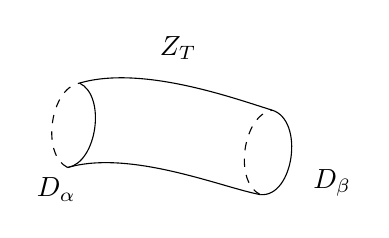
\begin{tikzpicture}[>=stealth,scale=0.95]
  \begin{scope}[rotate=-8]
  \draw (-1.0,0.62) .. controls (-0.2,0.98) and (1.1,0.70) .. (1.6,0.62);%
  \draw (-1.0,-0.52) .. controls (-0.2,-0.16) and (1.1,-0.50) .. (1.6,-0.52);%
  \draw (-1.0,0.62) .. controls (-0.62,0.5) and (-0.62,-0.4) .. (-1.0,-0.52);%
  \draw[dashed] (-1.0,-0.52) .. controls (-1.38,-0.4) and (-1.38,0.5) .. (-1.0,0.62);%
  \draw (1.6,0.62) .. controls (2.05,0.55) and (2.05,-0.50) .. (1.6,-0.52);%
  \draw[dashed] (1.6,-0.52) .. controls (1.22,-0.4) and (1.22,0.5) .. (1.6,0.62);%
  \node[above] at (0.28,0.98) {$Z_{T}$};
  \node[below] at (-1.15,-0.55) {$D_{\alpha}$};
  \node[right] at (2.15,-0.28) {$D_{\beta}$};
  \end{scope}
\end{tikzpicture}

图 6.8
\end{minipage}

在模型方程中不对 $L^{2}$-\trGradient{}作\trRegularization，我们便被引向
\begin{equation}\label{eq:ell-bvp-pde}
\begin{aligned}
&a_{s}\ +\ Ja_{t}\ =\ 0\qquad&&\text{于 }\mathring{D}\\
&u_{s}\ +\ Ju_{t}\ +\ H'(t,u)\ =\ 0\qquad&&\text{于 }(-T,T)\times S^{1}\\
&b_{s}\ -\ Jb_{t}\ =\ 0\qquad&&\text{于 }\mathring{D}\,,
\end{aligned}
\end{equation}
以及相配的\trBoundaryCondition{} \eqref{eq:ell-matching-bc}。我们将把方程组%
\eqref{eq:ell-bvp-pde} 连同\trBoundaryCondition{}改写成一个单独的方程。我们在%
\trCylinder{} $Z_{T}=[-T,T]\times S^{1}$ 的两端各添一个\textbf{\trCapDisk}（cap），以定义黎曼球面%
$S_{T}$，使得
\begin{equation}\label{eq:ell-sphere-st}
S_{T}\ =\ D\ \bigcup_{\alpha}\ Z_{T}\ \bigcup_{\beta}\ D\,.
\end{equation}
此处 $\alpha$ 与 $\beta$ 表示粘合等同
\[
\begin{aligned}
\alpha\ \ &:\ \ e^{2\pi it}\ \sim\ (-T,t)\\
\beta\ \ &:\ \ e^{-2\pi it}\ \sim\ (T,t)\,.
\end{aligned}
\]
接下来我们通过引入\trChart
\begin{equation}\label{eq:ell-charts-st}
\begin{aligned}
&\psi\ :\ (-T,T)\times S^{1}\ \longrightarrow\ \C\ :\ (s,t)\ \mapsto\ e^{2\pi(s+it)}\\
&\varphi_{1}\ :\ D\ \bigcup_{\alpha}\,[-T,0)\times S^{1}\ \longrightarrow\ \C\ :\ %
\left\{\begin{aligned}
&z\in D\ \mapsto\ z\\
&(s,t)\ \mapsto\ e^{2\pi(s+T+it)}
\end{aligned}\right.\\
&\varphi_{2}\ :\ (0,T]\times S^{1}\ \bigcup_{\beta}\,D\ \longrightarrow\ \C\ :\ %
\left\{\begin{aligned}
&z\in D\ \mapsto\ \bar{z}\\
&(s,t)\ \mapsto\ e^{2\pi(s-T+it)}
\end{aligned}\right.\,.
\end{aligned}
\end{equation}
来在 $S_{T}$ 上定义复\trManifold{}结构。我们观察到转移映射 $\varphi_{1}\circ\psi^{-1}$%
与 $\varphi_{2}\circ\psi^{-1}$ 是\trHolomorphic{}的。这些\trChart{}在 $S_{T}$ 上%
定义了一个\trComplexStructure{} $j$。由\trUniformization{}定理，$(S_{T},j)$ 双%
\trHolomorphic{}于 $(S^{2},i)$，此处 $S^{2}=\C\cup\{\infty\}$ 是标准的黎曼球面，%
例如参见 O.~\trForster{} [92]。为记号方便起见，我们把 $\alpha$-盘记作 $D_{1}$，把%
$\beta$-盘记作 $D_{2}$。现在考虑 $v\in C^{\infty}(S_{T},T^{2n})$，并定义映射%
$Lv$——它在 $\mathring{D}_{1}$、$\mathring{D}_{2}$ 与 $(-T,T)\times S^{1}$ 上%
\trSmooth——为
\begin{equation}\label{eq:ell-lv-torus}
Lv\ =\ Tv\ +\ J\circ(Tv)\circ j\ +\ \chi_{[-T,T]\times S^{1}}\Bigl(H'(v)\,ds\,-\,JH'(v)\,dt\Bigr)\,.
\end{equation}
此处 $(s,t)$ 是 $[-T,T]\times S^{1}$ 上的坐标，而 $\chi_{[-T,T]\times S^{1}}$ 是%
$S_{T}$ 上相应的示性函数。此外，$Tv$ 是映射 $v:S_{T}\to T^{2n}$ 的切映射。注意%
$(Lv)(z)$ 是一个线性映射 $T_{z}S_{T}\to T_{v(z)}T^{2n}$，它满足关系
\[
-J\circ\bigl(Lv\bigr)(z)\ =\ \bigl(Lv\bigr)(z)\circ j\,.
\]
我们以 $A_{T^{2n}}\to S_{T}\times T^{2n}$ 表示这样一个\trVectorBundle：其在%
$(z,m)$ 上的\trFiber{}由一切复反线性的映射 $\gamma:T_{z}S_{T}\to T_{m}T^{2n}$%
——即满足 $\gamma j=-J\gamma$ 者——组成。若 $v$ 是映射 $S_{T}\to T^{2n}$，我们以%
$v^{*}A_{T^{2n}}$ 表示借 $v$ 的图像 $z\mapsto(z,v(z))$ 而作的 $A_{T^{2n}}$ 的%
\trPullback。于是 $Lv$ 可以视为 $v^{*}A_{T^{2n}}\to S_{T}$ 的一个\trSection。%
设 $v$ 连续，且在 $S_{T}\setminus\bigl\{(\pm T,t)\,\big|\,t\in S^{1}\bigr\}$ 上%
\trSmooth，此外在两个圆周 $\{\pm T\}\times S^{1}$ 之外满足 $Lv=0$。这恰恰意味着%
$Lv$ 是 $v^{*}A_{T^{2n}}\to S_{T}$ 的\trZeroSection。考虑 $(-T,T)\times S^{1}$%
上的\trVectorField{} $\frac{\partial}{\partial s}$。那么
\[
\begin{aligned}
0\ &=\ \bigl(Lv\bigr)(s,t)\Bigl(\tfrac{\partial}{\partial s}\Bigr)\\
&=\ v_{s}\ +\ Jv_{t}\ +\ H'(t,v)\,.
\end{aligned}
\]
我们看到，$v$ 在 $(-T,T)\times S^{1}$ 上满足微分方程%
\eqref{eq:ell-bvp-pde}。在 $D_{1}$ 与 $D_{2}$ 上我们分别有 $v_{s}+Jv_{t}=0$ 与%
$v_{s}-Jv_{t}=0$。此外，在 $D_{1}$、$D_{2}$ 与 $[-T,T]\times S^{1}$ 的公共部分上%
\trBoundaryCondition{}也得到满足。

这一新构造可以容易地推广到任意\trCompact\trSymplecticManifold。为此，我们以 $j$%
表示 $S_{T}$ 上的\trComplexStructure，而以 $J$ 表示 $M$ 上一个与 $\omega$%
\trCompatible{}的\trAlmostComplexStructure。对映射 $v:S_{T}\to M$，我们定义%
$v^{*}A_{M}$ 的\trSection{} $Lv$ 为
\begin{equation}\label{eq:ell-lv-general}
\begin{aligned}
&(Lv)(z)\ =\ Tv(z)\ +\ J(v)\circ Tv(z)\circ j\\
&+\chi_{[-T,T]\times S^{1}}(z)\Bigl[H'\Bigl(t,v(z)\Bigr)\,ds\ -\ J\Bigl(v(z)\Bigr)H'\Bigl(t,v(z)\Bigr)\,dt\Bigr]\,.
\end{aligned}
\end{equation}
为了研究方程 $Lv=0$，我们需要建立一个合适的泛函分析框架。若 $2<p<\infty$，我们%
考虑由从 $S_{T}$ 到 $M$、属于\trSobolev{}类 $W^{1,p}$ 的映射构成的\trBanach{}流形%
$W^{1,p}(S_{T},M)$。关于 $W^{1,p}(S_{T},M)$ 上自然可微结构的构造，我们请读者参见%
H.~\trEliasson{} [79] 的文章。对 $v\in W^{1,p}(S_{T},M)$，我们考虑\trBundle{}%
$v^{*}A_{M}\to S_{T}$，并以 $L^{p}(v^{*}A_{M})$ 表示相伴的 $L^{p}$-\trSection{}%
空间。于是，我们可以给
\[
L^{p}\Bigl(W^{1,p}(S_{T},M)^{*}A_{M}\Bigr)\ =\ \bigcup_{v\in W^{1,p}(S_{T},M)}\bigl\{v\bigr\}\times L^{p}\bigl(v^{*}A_{M}\bigr)
\]
装备\trBanach{}空间丛的结构，其底为\trBanach{}流形 $W^{1,p}(S_{T},M)$。总括起来，%
我们已经把椭圆方程组 \eqref{eq:ell-bvp-pde} 连同相配的\trBoundaryCondition{}%
\eqref{eq:ell-matching-bc} 表述成这样一种形式：解要在\trBanach{}空间丛%
$L^{p}(W^{1,p}(S_{T},M)^{*}A_{M})\to W^{1,p}(S_{T},M)$ 的\trSection{} $L$ 的零点%
中寻找。我们将把解集记为
$X_{T}=\bigl\{\,v\in W^{1,p}(S_{T},M)\ \bigm|\ L(v)=0\,\bigr\}$。

注意，我们不能指望 $L(v)=0$ 的解 $v:S_{T}\to M$ 在\trCylinder{} $Z_{T}$ 的%
\trBoundary{} $\partial Z_{T}$ 附近具有优于 $W^{1,p}$ 的正则性。这是由于截断函数%
$s\mapsto\chi_{[-T,T]}(s)$ 在 $Z_{T}$ 的\trBoundary{}分支 $s=\pm T$ 处不%
\trSmooth{}所致。回顾一下，这两个\trBoundary{}分支与粘到\trCylinder{}上的两个%
\trDisc{} $D$ 的\trBoundary{}一致。然而，由附录 5 中的结果可以得知：$L(v)=0$ 的%
解 $v$ 除 $\partial Z_{T}$ 处外是\trSmooth{}的，在 $\partial Z_{T}$ 处 $s$ 方向%
（即垂直于诸\trBoundary{}的方向）的导数不相配。说得更精确些，由于 $p>2$，由%
\trSobolev{}嵌入定理我们有 $W^{1,p}(S_{T},M)\subset C^{0}(S_{T},M)$。于是连续的%
$v$ 可以在局部坐标中研究。若 $z$ 是\trCylinder{} $Z_{T}$ \trInterior{}中的一点，%
则在局部坐标中有 $v\in W^{1,p}(B_{\varepsilon},\R^{2n})$，此处 $B_{\varepsilon}$%
是以 $z$ 为中心的一个小开球。此外，$v$ 是一个特殊的一阶椭圆方程组的%
\trWeakSolution，于是由椭圆\trPartialDifferentialEquation{}的内部\trRegularity%
理论我们得出 $v\in C^{\infty}(B_{\varepsilon},\R^{2n})$。类似地，$L(v)$ 的解 $v$%
在诸\trDisc{} $D$ 的\trInterior{}中\trSmooth。附录 5 中证明了：此外，$v$ 从%
$Z_{T}$ 的\trInterior{}到其\trBoundary{} $\partial Z_{T}$ 有\trSmooth{}延拓，%
而且从诸\trDisc{}的\trInterior{}到它们的\trBoundary{}%
$\partial D_{1}\cup\partial D_{2}=\partial Z_{T}$ 也有\trSmooth{}延拓。这当然并%
不意味着诸解在\trBoundary{}处\trSmooth{}地拼合，因为垂直于\trBoundary{}的（$s$%
方向的）导数并不一致。但 $v$ 限制在\trBoundary{} $\partial Z_{T}$ 上是%
\trSmooth{}的，于是特别地，$v(-T)$ 与 $v(T)$ 是属于 $C^{\infty}_{c}(S^{1},M)$%
的\trSmooth\trLoop。

现在我们可以利用问题的变分结构，为诸解 $v\in X_{T}$ 导出一个自然的先验估计。%
回忆假设 $\omega\big|_{\pi_{2}(M)}=0$ 并设 $L(v)=0$。取常数 $C>0$ 使其同时界住%
$\bigl|\max_{(t,x)}H(t,x)\bigr|$ 与 $\bigl|\min_{(t,x)}H(t,x)\bigr|$。我们估计
\[
\begin{aligned}
\Phi_{H}\Bigl(v(-T)\Bigr)\ &=\ \int_{D_{1}}v^{*}\omega\ -\ \int_{0}^{1}H\Bigl(t,v(-T,t)\Bigr)\,dt\\
&\geq\ -\max_{(t,x)}H(t,x)\ \geq\ -C\,.
\end{aligned}
\]
这里用到了：对\trHolomorphic{}映射
\[
\int_{D_{1}}v^{*}\omega\ =\ \frac{1}{2}\int_{D_{1}}\bigl|\nabla v\bigr|^{2}_{J}\,ds\,dt\ \geq\ 0\,.
\]
类似地，
\[
\begin{aligned}
\Phi_{H}\Bigl(v(T)\Bigr)\ &=\ \int_{D_{2}}v^{*}\omega\ -\ \int_{0}^{1}H\Bigl(t,v(T,t)\Bigr)\,dt\\
&\leq\ -\min_{(t,x)}H(t,x)\ \leq\ C\,,
\end{aligned}
\]
这里用到：对反\trHolomorphic{}映射
\[
\int_{D_{2}}v^{*}\omega\ =\ -\frac{1}{2}\int_{D_{2}}\bigl|\nabla v\bigr|^{2}_{J}\ \leq\ 0\,.
\]
总括起来，我们证明了

\begin{lemma}\label{lem:action-tube-bound}
存在常数 $C>0$，它与 $T>0$ 无关，使得 $Lv=0$ 的每个解 $v:S_{T}\to M$ 满足
\[
-C\ \leq\ \Phi_{H}\Bigl(v(-T)\Bigr)\ \leq\ \Phi_{H}\Bigl(v(s)\Bigr)\ \leq\ \Phi_{H}\Bigl(v(T)\Bigr)\ \leq\ C\,,\qquad\text{对 }-T\leq s\leq T\,.
\]
\end{lemma}

由此我们得出

\begin{lemma}\label{lem:energy-estimate-zt}
存在常数 $C>0$，它与 $T>0$ 无关，使得 $Lv=0$ 的每个解%
$v\in W^{1,p}(S_{T},M)$ 满足
\[
\frac{1}{2}\int_{-T}^{T}\int_{0}^{1}\Bigl[\ \Bigl|\frac{\partial v}{\partial s}\Bigr|^{2}_{J}\ +\ \Bigl|\frac{\partial v}{\partial t}-X_{H_{t}}(v)\Bigr|^{2}_{J}\Bigr]\,ds\,dt\ \leq\ 2C\,.
\]
\end{lemma}

\begin{proof}
利用\cref{lem:action-tube-bound}，我们计算
\[
\begin{aligned}
2C\ \geq\ \Phi_{H}\Bigl(v(T)\Bigr)-\Phi_{H}\Bigl(v(-T)\Bigr)\ &=\ \int_{-T}^{T}\tfrac{d}{ds}\Phi_{H}\Bigl(v(s)\Bigr)\,ds\\
&=\ \int_{-T}^{T}\Bigl\|\Phi'_{H}\Bigl(v(s)\Bigr)\Bigr\|^{2}_{J,L^{2}}\,ds\\
&=\ \frac{1}{2}\int_{-T}^{T}\Bigl[\ \Bigl\|\tfrac{d}{ds}\,v(s)\Bigr\|^{2}_{J,L^{2}}\\
&\qquad\qquad+\ \Bigl\|\dot{v}(s)-X_{H}\Bigl(v(s)\Bigr)\Bigr\|^{2}_{J,L^{2}}\Bigr]\,ds\\
&=\ \frac{1}{2}\int_{-T}^{T}\int_{0}^{1}\Bigl[\ \Bigl|\tfrac{\partial v}{\partial s}(s,t)\Bigr|^{2}_{J}\\
&\qquad\qquad+\ \Bigl|\tfrac{\partial v}{\partial t}-X_{H_{t}}\Bigl(v(s,t)\Bigr)\Bigr|^{2}_{J}\Bigr]\,ds\,dt\,.
\end{aligned}
\]
此处 $\|\cdot\|_{J,L^{2}}$ 是借\trRiemann{}度量 $g_{J}$ 而得的诸\trSection{}的%
$L^{2}$-\trNorm。
\end{proof}

我们接下来的目标是研究由
\begin{equation}\label{eq:ell-xinfty-m-def}
\begin{aligned}
X_{\infty}=\Bigl\{\ &u\in C^{\infty}\bigl(\R\times S^{1},M\bigr)\ \Bigm|\ u_{s}+J(u)u_{t}\ +\ H'(t,u)=0\,,\\
&u(s)\in C^{\infty}_{c}(S^{1},M)\ \text{且}\ \Bigl(\Phi_{H}(u(s))\Bigr)_{s\in\R}\ \text{在 }\R\text{ 中有界}\Bigr\}\,.
\end{aligned}
\end{equation}
定义的「有界\trOrbit」空间 $X_{\infty}$ 的\trCompactness。我们注意到，%
为了后面的估计，方便的做法是借\trWhitney{}嵌入定理把 $M$ 视为某个 $\R^{N}$ 的%
\trCompact\trSubmanifold，例如参见 M.~\trHirsch{} [113]。由于%
$C^{\infty}(\R\times S^{1},\R^{N})$ 是一个带有通常平移不变度量 $d$ 的\trFrechet{}空间，%
我们可以把 $C^{\infty}(\R\times S^{1},M)$ 视为 $C^{\infty}(\R\times S^{1},\R^{N})$%
的一个闭子空间。诱导度量我们也记作 $d$。我们将会看到，$X_{\infty}$ 是%
$C^{\infty}(\R\times S^{1},\R^{N})$ 的一个\trCompact{}子空间。我们从下述命题开始：

\begin{proposition}\label{prop:critical-action-levels}
存在常数 $C>0$，使得对每个 $u\in X_{\infty}$ 都有
\[
\Phi_{H}\Bigl(u(s)\Bigr)\ \in\ [-C,C]\,,\qquad s\in\R\,.
\]
\end{proposition}

\begin{proof}
由假设，$\Phi_{H}(u(\R))$ 在 $\R$ 中有界。于是，缩记%
$\bigl\|\bigr\|=\bigl\|\bigr\|_{J,L^{2}}$，
\[
\int_{-\infty}^{+\infty}\Bigl\|\Phi'_{H}\Bigl(u(s)\Bigr)\Bigr\|^{2}\,ds\ =\ \int_{-\infty}^{+\infty}\Bigl(\frac{d}{ds}\Phi_{H}\bigl(u(s)\bigr)\Bigr)\,ds\ <\ +\infty\,.
\]
因此存在序列 $(s_{n})\subset\R$，$s_{n}\to+\infty$，使得
\[
\Phi_{H}\Bigl(u(s_{n})\Bigr)\ \longrightarrow\ \alpha\in\R\qquad\text{而}\qquad \Bigl\|\Phi'_{H}\Bigl(u(s_{n})\Bigr)\Bigr\|\ \longrightarrow\ 0\,.
\]
令 $x_{n}=u(s_{n})\in C^{\infty}(S^{1},M)$，我们得到
\begin{equation}\label{eq:ell-xdot-conv}
\bigl\|\dot{x}_{n}\,-\,X_{H}(x_{n})\bigr\|\ \longrightarrow\ 0\,.
\end{equation}
把 $x_{n}$ 视为映入 $\R^{N}$ 的映射，由 $M$ 的\trCompactness{}我们推出%
$\bigl\|\dot{x}_{n}\bigr\|_{L^{2}(S^{1},\R^{N})}\leq\operatorname{const}$，这里%
用了通常的 $L^{2}$-\trInnerProduct。于是我们可以找到子序列满足
\begin{equation}\label{eq:ell-weak-strong}
\begin{aligned}
x_{n}\ \rightharpoonup\ x\qquad&\text{在 }H^{1,2}(S^{1},\R^{N})\text{ 中弱收敛}\\
x_{n}\ \to\ x\qquad&\text{在 }C^{0}(S^{1},\R^{N})\text{ 中强收敛}\,.
\end{aligned}
\end{equation}
后一收敛由\trArzela-\trAscoli{}定理得出。由 \eqref{eq:ell-xdot-conv} 与%
\eqref{eq:ell-weak-strong} 我们得出：$\dot{x}_{n}$ 是 $L^{2}$ 中的柯西序列，从而
\begin{equation}\label{eq:ell-hn-h12}
x_{n}\ \to\ x\ \text{于 }H^{1,2}(S^{1},M)\text{ 中}\,,\qquad \dot{x}\ =\ X_{H}(x)\,.
\end{equation}
因此 $x\in C^{\infty}(S^{1},M)$，且 $x$ 是该\trHamiltonianVectorField{}的一个%
$1$-\trPeriodicSolution。现在 $\Phi_{H}(x_{n})\to\Phi_{H}(x)$，故%
$\alpha=\Phi_{H}(x)$。对 $s_{n}\to-\infty$ 的序列 $x_{n}=u(s_{n})$ 可以类似地%
论证。由\trArzela-\trAscoli{}定理，全体 $1$-\trPeriodicSolution{}%
$\dot{x}=X_{H}(x)$ 之集在 $C^{\infty}(S^{1},\R^{N})$ 中\trCompact，从而临界%
水平之集
\[
\mathcal{C}:=\Bigl\{\ \Phi_{H}(x)\ \Bigm|\ \Phi'_{H}(x)\ =\ 0\ \Bigr\}
\]
在 $\R$ 中\trCompact。我们取 $C>0$ 充分大使得区间 $[-C,C]$ 含有 $\mathcal{C}$。%
由于 $s\to\Phi_{H}(u(s))$ \trMonotone，而且如我们所见，\trBounded{}解 $u$ 连接%
诸\trCriticalPoint，我们得出：对一切 $s\in\R$ 有%
$-C\leq\Phi_{H}(u(s))\leq C$，命题得证。
\end{proof}

\begin{corollary}\label{cor:xinfty-closed}
$X_{\infty}$ 在 $C^{\infty}(\R\times S^{1},M)$ 中是闭的。
\end{corollary}

\begin{proof}
任取序列 $(u_{n})\subset X_{\infty}$。由\cref{prop:critical-action-levels}我们%
知道 $\Phi_{H}(u_{n}(\R))\subset[-C,C]$。设 $u_{n}$ 按 $C^{\infty}$-度量 $d$%
收敛于 $u$。对每个 $r>0$ 我们得到
\[
C\ \geq\ \Phi_{H}\Bigl(u_{n}(r)\Bigr)\ \geq\ \Phi_{H}\Bigl(u_{n}(-r)\Bigr)\ \geq\ -C\,.
\]
于是，当 $n\to\infty$ 时这一估计蕴含 $\Phi_{H}(u(\R))\subset\R$ 有界。此外，%
由于 $\frac{\partial u_{n}}{\partial s}+J(u_{n})\frac{\partial u_{n}}{\partial t}+H'(t,u_{n})=0$，%
我们可以取极限并看到 $u$ 也满足该微分方程。这表明确实如所断言 $u\in X_{\infty}$。
\end{proof}

几何图景与 6.2 节中一样：一条「有界\trOrbit」$u\in X_{\infty}$ 连接 $M$ 上%
\trHamiltonianEquation{} $\dot{x}=X_{H}(x)$ 的诸 $1$-\trPeriodicSolution。%
接下来我们证明 $X_{\infty}$ 是 $C^{\infty}(\R\times S^{1},M)$ 的一个%
\trCompact{}子集。注意，度量空间 $C^{\infty}(\R\times S^{1},M)$ 具有\trHeine-%
\trBorel{}性质；这是把\trArzela-\trAscoli{}定理应用到函数的各阶导数上的一个%
推论。既然由上述推论可知 $X_{\infty}$ 是闭集，我们只须证明%
$X_{\infty}\subset C^{\infty}(\R\times S^{1},M)$ 有界。这就要求：对每个%
\trCompact{}集 $K\subset\R\times S^{1}$ 与每个整数 $n\in\mathbb{N}$，存在常数%
$C_{K,n}>0$，使得
\begin{equation}\label{eq:ell-derivative-bound}
\sup_{\scriptstyle(s,t)\in K\atop\scriptstyle|\alpha|\leq n}\ \bigl|D^{\alpha}u(s,t)\bigr|\ \leq\ C_{K,n}\qquad\text{对一切 }u\in X_{\infty}\,.
\end{equation}
\eqref{eq:ell-derivative-bound} 之证明的关键成分是一个对 $u\in X_{\infty}$ 一致%
的\trGradient{}估计。这里我们将在关键之处用到假设%
$\omega\big|_{\pi_{2}(M)}=0$。注意，为了能在局部坐标中工作，我们必须确保：对%
整族映射而言，一个点的固定的局部\trNeighborhood{}被映入像空间的同一个\trChart。

\begin{theorem}\label{thm:gradient-estimate}
设 $\omega\big|_{\pi_{2}(M)}=0$。那么存在常数 $A>0$，使得
\[
\bigl|\nabla u(s,t)\bigr|_{J}\ \leq\ A
\]
对一切 $u\in X_{\infty}$ 与 $(s,t)\in\R\times S^{1}$ 成立。
\end{theorem}

\begin{proof}
反证：我们找到序列 $(s_{k},t_{k})\in\R\times S^{1}$ 与 $(u_{k})\subset X_{\infty}$，%
使得
\[
\bigl|\nabla u_{k}(s_{k},t_{k})\bigr|_{J}\ \longrightarrow\ +\infty\,.
\]
由于 $X_{\infty}$ 在 $\R$-作用 \eqref{eq:ell-rinfty-action} 下\trInvariant，%
我们可以把 $u_{k}$ 换成 $u_{k}\cdot s_{k}$ 而设 $s_{k}=0$。此外，取子序列后可设%
$t_{k}\to t_{0}$。任取满足
\begin{equation}\label{eq:ell-epsilon-blowup}
\varepsilon_{k}>0\ ,\ \varepsilon_{k}\to0\ ,\ \varepsilon_{k}\bigl|(\nabla u_{k})(s_{k},t_{k})\bigr|_{J}\ \longrightarrow\ +\infty\,.
\end{equation}
的序列 $(\varepsilon_{k})$。我们希望这个序列还满足一些附加条件，并使用一个小%
技巧。它基于下述引理：

\begin{lemma}\label{lem:doubling-trick}
设 $(X,d)$ 是完备度量空间，$g:X\to[0,+\infty)$ 是连续映射。设给定%
$x_{0}\in X$ 与 $\varepsilon_{0}>0$。那么存在 $x\in X$ 与 $\varepsilon>0$，%
使得
\[
\begin{aligned}
&0<\varepsilon\ \leq\ \varepsilon_{0}\\
&g(x)\varepsilon\ \geq\ g(x_{0})\varepsilon_{0}\\
&d(x,x_{0})\ \leq\ 2\varepsilon_{0}\\
&g(y)\ \leq\ 2g(x)\qquad\text{对一切满足 }d(y,x)\leq\varepsilon\text{ 的 }y\,.
\end{aligned}
\]
\end{lemma}

\begin{proof}[\cref*{lem:doubling-trick}的证明]
假设不存在满足 $d(x_{1},x_{0})\leq\varepsilon_{0}$ 且 $g(x_{1})>2g(x_{0})$ 的%
$x_{1}\in X$。那么取 $x=x_{0}$ 与 $\varepsilon=\varepsilon_{0}$ 即得结论。%
否则我们可以取这样一个 $x_{1}$，并且归纳地进行：可以假设存在%
$x_{0},x_{1},\ldots,x_{n}$ 满足
\[
d(x_{k},x_{k-1})\ \leq\ \frac{\varepsilon_{0}}{2^{k-1}}\qquad\text{而}\qquad g(x_{k})>2g(x_{k-1})
\]
对一切 $1\leq k\leq n$。那么，若不存在满足
\begin{equation}\label{eq:ell-induction-step}
d(x_{n+1},x_{n})\ \leq\ \frac{\varepsilon_{0}}{2^{n}}\quad\text{而}\quad g(x_{n+1})>2g(x_{n})\,,
\end{equation}
的 $x_{n+1}$，则取 $x=x_{n}$ 与 $\varepsilon=\frac{\varepsilon_{0}}{2^{n}}$ 即得%
结论。的确，$x_{n}$ 满足%
$d(x_{n},x_{0})\leq d(x_{n},x_{n-1})+\cdots+d(x_{1},x_{0})\leq2\varepsilon_{0}$，%
而 $g(x_{n})>2g(x_{n-1})>2^{2}g(x_{n-2})>2^{n}g(x_{0})$，于是%
$g(x_{n})\varepsilon>g(x_{0})\varepsilon_{0}$。此外，由%
\eqref{eq:ell-induction-step} 我们得出：若 $d(y,x_{n})\leq\varepsilon$，则%
$g(y)\leq2g(x_{n})$\footnote{原书印作「$g(y_{n})\leq 2g(x_{n})$」，其 $y_{n}$ 疑为「$y$」之误，此处径改。——译者注}，断言得证。另一方面，若存在满足%
\eqref{eq:ell-induction-step} 的 $x_{n+1}$，我们就继续这一过程。它必定在有限多%
步之后终止，因为否则我们就有满足 $g(x_{n})\to+\infty$ 的柯西序列%
$(x_{n})\subset X$。这是不可能的，因为 $x_{n}\to x^{*}$ 而 $g$ 在 $x^{*}$ 处%
连续。
\end{proof}

为简化记号，下文中我们将以 $|\cdot|$ 代替切空间上的\trRiemann{}\trNorm{}%
$|\cdot|_{J}$。鉴于上述引理，我们可以把 $x_{k}=(s_{k},t_{k})$ 与 $\varepsilon_{k}$%
换成稍有修改的序列，并且（再次利用 $\R$-作用）可以假设上述序列 $u_{k}$ 还满足
\begin{equation}\label{eq:ell-gradient-double}
\bigl|\nabla u_{k}(s,t)\bigr|\ \leq\ 2\bigl|\nabla u_{k}(0,t_{k})\bigr|\,,\qquad\text{若 }|s|^{2}+|t-t_{k}|^{2}\leq\varepsilon_{k}^{2}\,,\ 0\leq t_{k}\leq1\,.
\end{equation}
这里我们方便地把诸映射 $u$ 视为通过 $t$ 变量的 $1$-周期延拓而定义在%
$\R\times\R$ 上的映射。经重新标度，我们定义新序列 $v_{k}\in C^{\infty}(\R^{2},M)$%
为
\begin{equation}\label{eq:ell-rescaled-vk}
v_{k}(s,t)\ =\ u_{k}\Bigl((0,t_{k})\ +\ \frac{1}{R_{k}}(s,t)\Bigr)\,,\qquad\text{此处 }R_{k}\ =\ \bigl|\nabla u_{k}(0,t_{k})\bigr|\,.
\end{equation}
以 $D_{k}$ 表示「大」\trDisc{}%
$D_{k}=\bigl\{\,x=(s,t)\in\R^{2}\ \bigm|\ |x|\leq\varepsilon_{k}R_{k}\,\bigr\}\subset\R^{2}$。%
那么序列 $v_{k}$ 具有下述性质：
\begin{equation}\label{eq:ell-vk-properties}
\begin{gathered}
v_{k}\in C^{\infty}(D_{k},M)\\
\bigl|\nabla v_{k}(x)\bigr|\ \leq\ 2\qquad\text{对 }x\in D_{k}\\
\bigl|\nabla v_{k}(0)\bigr|\ =\ 1\\
\varepsilon_{k}R_{k}\ \longrightarrow\ +\infty\,.
\end{gathered}
\end{equation}
此外，$v_{k}$ 满足\trPartialDifferentialEquation
\begin{equation}\label{eq:ell-vk-pde}
\frac{\partial}{\partial s}\,v_{k}\ +\ J(v_{k})\frac{\partial}{\partial t}\,v_{k}\ =\ -\frac{1}{R_{k}}\,H'\Bigl(t_{k}+\frac{t}{R_{k}}\,,\,v_{k}\Bigr)
\end{equation}
于 $D_{k}$ 上。由于 $u_{k}\in X_{\infty}$，鉴于\cref{lem:energy-estimate-zt}我们%
得到
\begin{equation}\label{eq:ell-vk-area}
\int_{D_{k}}\bigl|\nabla v_{k}\bigr|^{2}\,ds\,dt\ \leq\ 13C\,,
\end{equation}
对大的 $k$，其中 $C>0$ 是\cref{lem:energy-estimate-zt}中的普适常数。的确，引入%
「小」\trDisc{} $B_{k}=B_{\varepsilon_{k}}(0,t_{k})\subset\R^{2}$，我们得到
\[
\begin{aligned}
&\int_{D_{k}}\bigl|\nabla v_{k}\bigr|^{2}\,ds\,dt\ =\ \int_{B_{k}}\bigl|\nabla u_{k}\bigr|^{2}\,ds\,dt\\
&=\ \int_{B_{k}}\Bigl\{\ \Bigl|\frac{\partial u_{k}}{\partial s}\Bigr|^{2}\ +\ \Bigl|\frac{\partial u_{k}}{\partial t}-X_{H}(u_{k})\ +\ X_{H}(u_{k})\Bigr|^{2}\Bigr\}\,ds\,dt\\
&\leq\ 3\int_{B_{k}}\Bigl|\frac{\partial u_{k}}{\partial s}\Bigr|^{2}\,ds\,dt\ +\ 2\int_{B_{k}}\Bigl|X_{H}(u_{k})\Bigr|^{2}\,ds\,dt\\
&\leq\ 3\int_{\R\times S^{1}}\Bigl|\frac{\partial u_{k}}{\partial s}\Bigr|^{2}\,ds\,dt\ +\ l_{k}\ \leq\ 12C\ +\ l_{k}\,,
\end{aligned}
\]
其中当 $k\to\infty$ 时 $l_{k}\to0$。这就证明了断言%
\eqref{eq:ell-vk-area}。由于 $v_{k}$ 的\trGradient{}一致有界，我们稍后将由%
方程 \eqref{eq:ell-vk-pde} 的椭圆估计得出下述至关重要的结论：

\begin{lemma}\label{lem:holomorphic-convergence}
设序列 $v_{k}$ 满足 \eqref{eq:ell-vk-properties} 与%
\eqref{eq:ell-vk-pde}。那么存在 $v\in C^{\infty}(\R^{2},M)$ 与一个子序列，%
使得
\[
v_{k}\ \to\ v\qquad\text{于 }C^{\infty}(\R^{2},M)\text{ 中}\,.
\]
\end{lemma}

我们把这一引理的证明搁置一下，接下来展示\cref{thm:gradient-estimate}如何由我们的%
拓扑假设 $[\omega]\big|_{\pi_{2}(M)}=0$ 得出。我们观察到该引理所保证的%
\trSmooth{}映射 $v$ 是一个面积有限且为正的\trHolomorphic{}映射，因而不是常值%
映射。的确，由 \eqref{eq:ell-vk-properties}、\eqref{eq:ell-vk-pde} 与%
\eqref{eq:ell-vk-area} 我们推出 $v$ 的下述性质：
\begin{equation}\label{eq:ell-v-properties}
\begin{gathered}
\bigl|\nabla v(0)\bigr|\ =\ 1\\
\bigl|\nabla v(x)\bigr|\ \leq\ 2\,,\qquad x\in\R^{2}\\
v_{s}\ +\ J(v)v_{t}\ =\ 0\\
0<\Bigl|\ \int_{\R^{2}}v^{*}\omega\Bigr|\ =\ \frac{1}{2}\int_{\R^{2}}\Bigl|\nabla v\Bigr|^{2}\ <\ \infty\,.
\end{gathered}
\end{equation}
对 $R>0$ 定义单调函数 $\Phi(R)$ 为
\begin{equation}\label{eq:ell-monotone-phi}
\Phi(R):=\Bigl|\ \int_{D_{R}}v^{*}\omega\Bigr|\ =\ \frac{1}{2}\int_{D_{R}}\bigl|\nabla v\bigr|^{2}\ \nearrow\ \frac{1}{2}\int_{\R^{2}}\bigl|\nabla v\bigr|^{2}\,.
\end{equation}
\trHolomorphic\trDisc{} $v\big|_{D_{R}}:D_{R}\to M$ 限制到\trBoundary{}上，借%
$x_{R}(\tau)=v(Re^{2\pi i\tau})$ 定义了可缩\trLoop{} $x_{R}:S^{1}\to M$。鉴于%
\eqref{eq:ell-v-properties} 中的微分方程，这条\trLoop{}满足%
$\bigl|\dot{x}_{R}(\tau)\bigr|=2\pi R\,\Bigl|\tfrac{\partial v}{\partial s}(Re^{2\pi i\tau})\Bigr|$。%
用极坐标计算我们得到
\[
\int_{\R^{2}}\Bigl|\frac{\partial v}{\partial s}\Bigr|^{2}\ =\ \int_{0}^{\infty}\frac{1}{2\pi R}\int_{0}^{1}\bigl|\dot{x}_{R}(\tau)\bigr|^{2}\,d\tau\,dR\,,
\]
由 \eqref{eq:ell-v-properties} 它是有限的。于是，存在一列\trHolomorphic\trDisc%
$v\big|_{D_{R_{j}}}$，使得其\trBoundary{}的弧长 $l(x_{R_{j}})$ 当 $j\to\infty$ 时%
趋于零。为了用弧长估计这些\trDisc{}的面积，我们用有限多个开集 $U_{j}\subset M$%
（$1\leq j\leq N$）覆盖\trCompact\trManifold{} $M$，使得每个 $\bar{U}_{j}$%
\trDiffeomorphic{}于一个闭球。存在常数 $d>0$，使得 $M$ 上直径 $\leq d$ 的每条%
\trLoop{}都含于某个集合 $U_{j}$。由\trPoincare{}引理我们得出：%
$\omega\big|_{\bar{U}_{j}}=d\lambda_{j}$，其中 $\lambda_{j}$ 是 $\bar{U}_{j}$ 上的%
一个 $1$-\trOneForm。因此我们可以用弧长 $l(x)$ 来估计\trLoop{}%
$x(t)\subset U_{j}$（$t\in[0,1]$）的\trAction：
\begin{equation}\label{eq:ell-action-loop-bound}
\Bigl|\ \int_{[0,1]}x^{*}\lambda_{j}\Bigr|\ \leq\ l(x)\,\bigl|\bigl|\lambda_{j}\bigr|\bigr|\,,
\end{equation}
其中 $\bigl|\bigl|\lambda_{j}\bigr|\bigr|=\max\bigl\{\,\bigl|\bigl|\lambda_{j}(m)\bigr|\bigr|\ ,\ m\in\bar{U}_{j}\,\bigr\}$\footnote{原书此句两处印作「$\bigl|\bigl|\lambda_{J}\bigr|\bigr|$」，其下标 $J$ 疑为「$j$」之误（两处同），此处径改小写。——译者注}，%
这里的\trNorm{}是线性映射 $\lambda_{j}(m)\in(T_{m}M)^{*}$ 的标准\trNorm。于是，%
若 $\gamma=\max\bigl\{\,\bigl|\bigl|\lambda_{j}\bigr|\bigr|\ ,\ 1\leq j\leq N\,\bigr\}$，%
则对 $M$ 上直径 $\leq d$ 的每条\trLoop{} $x$ 我们得出
\begin{equation}\label{eq:ell-action-loop-gamma}
\Bigl|\ \int_{x}\lambda_{j}\Bigr|\ \leq\ l(x)\cdot\gamma\,.
\end{equation}
现在考虑小\trLoop{} $x_{R}(\tau)$，它是\trHolomorphic\trDisc{} $v_{R}$ 的%
\trBoundary。那么它含于某个开集，比如说 $U_{j}$ 之中。由于它可缩，我们可以选取%
另一个\trDisc{} $w:D_{R}\to M$，它也满足 $w\big|_{\partial D}=x_{R}$，此外还含于%
$U_{j}$ 之中，从而 $w(D_{R})\subset U_{j}$。例如，若%
$\alpha:\bar{U}_{j}\to\overline{B_{1}(0)}\subset\R^{2n}$ 是一个局部\trChart，%
我们就用%
$w\bigl(re^{2\pi i\vartheta}\bigr)=\alpha^{-1}\Bigl(\frac{r}{R}\,\alpha\circ v(Re^{2\pi i\vartheta})\Bigr)$%
来定义这样一个\trDisc。

\noindent\begin{minipage}{\linewidth}
\centering
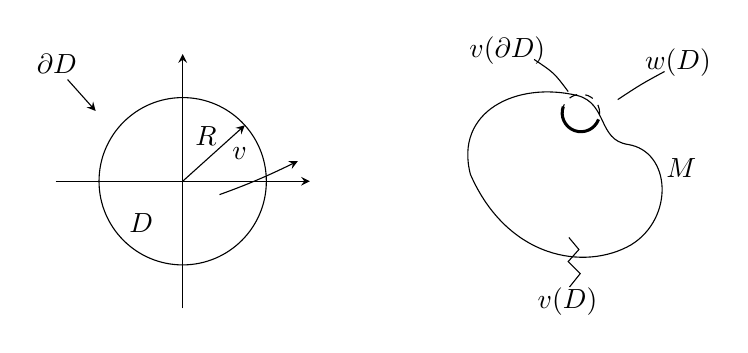
\begin{tikzpicture}[>=stealth,scale=0.85]
  \draw[->] (-1.9,0) -- (1.9,0);
  \draw[->] (0,-1.9) -- (0,1.9);
  \node at (0.65,1.62) {$\C$};
  \draw (0,0) circle (1.25);
  \draw[->] (0,0) -- (42:1.25);
  \node at (0.35,0.68) {$R$};
  \node at (-0.62,-0.62) {$D$};
  \draw[->] (-1.72,1.52) -- (-1.3,1.05);%
  \node at (-1.88,1.75) {$\partial D$};
  \draw[->] (0.55,-0.2) .. controls (1.05,-0.02) and (1.35,0.12) .. (1.72,0.3);%
  \node at (0.85,0.42) {$v$};
  \draw (4.3,0.1) .. controls (4.05,1.05) and (5.0,1.5) .. (5.9,1.28)
        .. controls (6.35,1.16) and (6.2,0.62) .. (6.65,0.55)
        .. controls (7.3,0.45) and (7.35,-0.55) .. (6.7,-0.95)
        .. controls (6.0,-1.35) and (4.85,-1.15) .. (4.3,0.1);%
  \draw[dashed] (5.95,1.02) circle (0.28);%
  \draw[line width=1.1pt] (5.95,1.02) ++(160:0.28) arc (160:340:0.28);%
  \node at (4.85,1.95) {$v(\partial D)$};
  \draw (5.25,1.82) .. controls (5.55,1.62) .. (5.76,1.34);%
  \node at (7.4,1.78) {$w(D)$};
  \draw (7.2,1.64) .. controls (6.85,1.45) .. (6.5,1.22);%
  \node at (7.45,0.2) {$M$};
  \node at (5.75,-1.8) {$v(D)$};
  \draw (5.78,-1.58) -- (5.94,-1.38) -- (5.76,-1.2) -- (5.92,-1.02) -- (5.77,-0.84);%
\end{tikzpicture}

图 6.9
\end{minipage}

最后我们来耍一张王牌。由于 $[\omega]\big|_{\pi_{2}(M)}=0$，对诸\trDisc{}%
$v\big|_{D_{R}}$ 与 $w$ 我们得出
\begin{equation}\label{eq:ell-equal-periods}
\int_{D_{R}}v^{*}\omega\ =\ \int_{D_{R}}w^{*}\,\omega\,.
\end{equation}
于是，在 $U_{j}$ 中应用\trStokes{}定理，鉴于%
\eqref{eq:ell-action-loop-gamma} 我们得到
\[
\Phi(R)\ =\ \Bigl|\ \int_{D_{R}}v^{*}\omega\Bigr|\ =\ \Bigl|\ \int_{[0,1]}x_{R}^{*}\lambda_{j}\Bigr|\ \leq\ l(x_{R})\cdot\gamma\,.
\]
然而，正如上面所见，存在\trHolomorphic\trDisc{}的序列使 $l(x_{R_{j}})\to0$，%
于是我们与 $\Phi(R)$ 的单调性 \eqref{eq:ell-monotone-phi} 相矛盾。这一矛盾表明%
我们的假设——即 $u\in X_{\infty}$ 的\trGradient{}不一致有界——为假。于是%
\cref{thm:gradient-estimate}为真。

上述技巧通常被称为\trBubblingOffAnalysis。为完成%
\cref{thm:gradient-estimate} 的证明，尚须证明%
\cref{lem:holomorphic-convergence}。

\begin{proof}[\cref*{lem:holomorphic-convergence}的证明]
为了简化程序，我们先把 \eqref{eq:ell-vk-pde} 中的\trHamiltonian{}项——它当%
$R_{k}\to\infty$ 时趋于零——去掉。借助 M.~\trGromov{} [107] 的一个技巧，令%
$\tilde{u}=(s,t,m)\in\R^{2}\times M$，并定义%
$J_{k}:T(\R^{2}\times M)\to T(\R^{2}\times M)$ 为
\begin{equation}\label{eq:ell-jk-structure}
J_{k}(\tilde{u})(\alpha,\beta,h)\ =\ \Bigl(\,-\beta\,,\ \alpha\,,\ J(m)h\ +\ \beta H'_{k}(t,m)\ +\ \alpha J(m)H'_{k}(t,m)\Bigr)\,,
\end{equation}
其中 $H'_{k}(t,m)=\frac{1}{R_{k}}H'\Bigl(t_{k}+\frac{t}{R_{k}}\,,m\Bigr)$。%
容易验证 $J_{k}^{2}=-\id$。于是，若按通常方式把 $\R^{2}$ 等同于 $\C$，则 $J_{k}$%
是 $\R^{2}\times M$ 上的一列\trAlmostComplexStructure，它连同其全部导数在%
$\R^{2}\times M$ 上一致收敛到\trAlmostComplexStructure{} $i\oplus J$。定义序列%
$\tilde{v}_{k}\in C^{\infty}(D_{k},\R^{2}\times M)$\footnote{原书印作%
「$C^{\infty}(\R^{2},\R^{2}\times M)$」，然 $v_{k}$（从而 $\tilde{v}_{k}$）只在%
逐渐扩大的圆盘 $D_{k}$ 上有定义，其诸性质亦仅在 $D_{k}$ 上列出，此处径改。%
——译者注} 为
\begin{equation}\label{eq:ell-tilde-vk}
\tilde{v}_{k}(s,t)\ =\ \Bigl(s,t,v_{k}(s,t)\Bigr)\,.
\end{equation}
那么，在 $D_{k}=B_{\varepsilon_{k}R_{k}}(0)\subset\R^{2}$ 上，
\begin{equation}\label{eq:ell-tilde-vk-props}
\begin{gathered}
\frac{\partial}{\partial s}\tilde{v}_{k}\ +\ J_{k}(\tilde{v}_{k})\frac{\partial}{\partial t}\tilde{v}_{k}\ =\ 0\\
\bigl|\nabla\tilde{v}_{k}(s,t)\bigr|\ \ \leq\ \ 4\\
\bigl|\nabla\tilde{v}_{k}(0,0)\bigr|\ \ \geq\ \ 1\\
\varepsilon_{k}R_{k}\ \to\ \infty\,.
\end{gathered}
\end{equation}
目标是找到一个子序列，使得 $\tilde{v}_{k}\to\tilde{v}$ 在渐扩的诸定义域%
$D_{k}$ 上于 $C^{\infty}$ 意义下局部收敛（对每个固定的\trCompact{}集，当 $k$ 充分大时），其中%
$\tilde{v}\in C^{\infty}(\R^{2},\R^{2}\times M)$。鉴于\trArzela-\trAscoli{}定理，%
只须找到 $\tilde{v}_{k}$ 的 $C^{\infty}_{\mathrm{loc}}$-界，也就是说，对每个%
\trCompact{}集 $K$，我们必须找到对 $k$ 一致的、$v_{k}$ 连同其全部导数的界。取%
$p>2$，鉴于\trSobolev{}嵌入定理，只须在每个\trCompact{}子集 $K\subset\R^{2}$ 上%
建立对所有 $l\geq1$ 的、一致的 $W^{l,p}(K)$ 界，以代替 $C^{l}(K)$ 界。为了建立%
这样的 $W^{l,p}_{\mathrm{loc}}$-界，我们归纳地进行。由假设，$\tilde{v}_{k}$ 的%
\trGradient{}一致有界，故 $W^{1,p}_{\mathrm{loc}}$-界有保证。反证：现在假设对%
某个 $l\geq1$ 有 $W^{l,p}_{\mathrm{loc}}$-界但没有%
$W^{l+1,p}_{\mathrm{loc}}$-界。于是，可能取 $\tilde{v}_{k}$ 的一个子序列后，我们%
找到序列 $x_{k}\in\R^{2}$ 与序列 $\varepsilon_{k}>0$，$\varepsilon_{k}\to0$，%
满足
\begin{equation}\label{eq:ell-blowup-sequence}
x_{k}\ \to\ x_{0}\qquad\text{而}\qquad \bigl|\tilde{v}_{k}\bigr|_{W^{l+1,p}\left(B_{\varepsilon_{k}}(x_{k})\right)}\ \to\ +\infty\,,
\end{equation}
此处把 $\R^{2}\times M$ 嵌入某个 $\R^{N}$，并把 $\tilde{v}_{k}:D_{k}\to\R^{N}$%
视为欧氏值的映射。由假设 $|\nabla\tilde{v}_{k}|$ 一致有界，故由%
\trArzela-\trAscoli{}定理可知，取一子列后有
\begin{equation}\label{eq:ell-conv-c0loc}
\tilde{v}_{k}(x_{0})\ \to\ (x_{0},m)\qquad\text{而}\qquad \tilde{v}_{k}\ \to\ \tilde{v}\quad\text{于 }C^{0}_{\mathrm{loc}}\text{ 中}\,.
\end{equation}
这使我们能把问题局部化到一个坐标卡中。围绕 $(x_{0},m)\in\R^{2}\times M$ 有一个%
\trChart{} $\alpha:U\to\R^{2+2n}$，满足 $\alpha(x_{0},m)=0$，且
\begin{equation}\label{eq:ell-localize-chart}
\tilde{v}_{k}\Bigl(\overline{B_{\varepsilon_{0}}(x_{0})}\Bigr)\ \subset\ V\ \subset\ \bar{V}\ \subset\ U\,,
\end{equation}
对某个 $\varepsilon_{0}>0$、$(x_{0},m)$ 的一个合适的开\trNeighborhood{} $V$ 以及%
一切充分大的 $k$ 成立。于是，定义\trSmooth{}函数%
$u_{k}:=\alpha\circ\tilde{v}_{k}:\overline{B_{\varepsilon_{0}}(x_{0})}\to\R^{2+2n}$\footnote{原书印作「$\overline{B_{\varepsilon_{0}}}(x,0)$」，依 \eqref{eq:ell-localize-chart} 其 $(x,0)$ 当为「$x_{0}$」，此处径改。——译者注}，%
并把 $J_{k}$ 换成由
\begin{equation}\label{eq:ell-jhat-k}
\hat{J}_{k}(y)\ =\ T\alpha\Bigl(\alpha^{-1}(y)\Bigr)\cdot J_{k}\Bigl(\alpha^{-1}(y)\Bigr)T\alpha^{-1}(y)\,,
\end{equation}
（$y\in\alpha(U)\subset\R^{2+2n}$）定义的 $\hat{J}_{k}$，我们在%
$B_{\varepsilon_{0}}(x_{0})$ 上便有
\begin{equation}\label{eq:ell-uk-props}
\begin{gathered}
\frac{\partial u_{k}}{\partial s}\ +\ \hat{J}_{k}(u_{k})\frac{\partial u_{k}}{\partial t}\ =\ 0\\
u_{k}(x_{0})\ \ \to\ \ 0\\
\bigl|\nabla u_{k}(x)\bigr|\ \ \leq\ \ C\\
\bigl|u_{k}\bigr|_{W^{l+1,p}\left(B_{\varepsilon_{k}}(x_{k})\right)}\ \ \to\ \ +\infty\,.\text{\footnote{原书印作「$B_{\varepsilon_{0}}(x_{k})$」，依假设 \eqref{eq:ell-blowup-sequence} 当为缩小的球「$B_{\varepsilon_{k}}(x_{k})$」，且证明结尾仅在此缩小球上取得矛盾，此处径改。——译者注}}
\end{gathered}
\end{equation}
此外，$\hat{J}_{k}\to\hat{J}_{\infty}$（于 $C^{\infty}$ 中），其中%
$\hat{J}_{\infty}$ 是 $\R^{2+2n}$ 中 $0$ 附近的某个\trAlmostComplexStructure。%
我们把 $\R^{2+2n}$ 上下述常值复结构记作 $J_{0}$：
\[
J_{0}:=\hat{J}_{\infty}(0)\,,\qquad J_{0}^{2}\ =\ -\mathbf{1}\,.
\]
现在我们利用\trCauchy-\trRiemann\trOperator{}的下述众所周知的椭圆估计。对每个%
$1<p<\infty$、$m$ 与 $n\geq0$，存在常数 $C>0$，使得
\begin{equation}\label{eq:ell-cr-estimate}
C\bigl|u\bigr|_{m+1,p}\ \leq\ \bigl|u_{s}\ +\ J_{0}u_{t}\bigr|_{m,p}\,,
\end{equation}
对每个在\trUnitBall{}中具\trCompactSupport{}的\trSmooth{}函数%
$u:\R^{2}\to\R^{2n+2}$ 成立。这是（用复记号写出时的）\trCauchy-\trRiemann%
\trOperator{}的经典估计，此处 $J_{0}$ 为常值。关于证明，我们参考 E.~\trStein{} [205]%
的专著第 60 页。为了应用这一估计，取\trSmooth{}函数 $\beta:\R^{2}\to[0,1]$\footnote{原书印作「$\beta:\R\to[0,1]$」，然下文以 $\beta\Bigl(\frac{x-x_{0}}{\lambda}\Bigr)$ 作用于二维变量并论单位圆盘支集，当为「$\beta:\R^{2}\to[0,1]$」，此处径改。——译者注}，使得%
$\beta(s)=1$（当 $|s|\leq\frac{1}{2}$）而 $\beta(s)=0$（当 $|s|\geq1$）。对%
$\lambda>0$ 定义函数 $\alpha_{\lambda}(x):=\beta\Bigl(\frac{x-x_{0}}{\lambda}\Bigr)$。%
那么若 $|x-x_{0}|\geq\lambda$ 则 $\alpha_{\lambda}(x)=0$。为简化公式，我们将%
使用缩记
\[
\bigl|u\bigr|_{l}\ :=\ \bigl|u\bigr|_{W^{l,p}\left(B_{\varepsilon_{0}}(x_{0})\right)}\,,
\]
其中 $p>2$ 已固定。此外，我们把 $\alpha\equiv\alpha_{\lambda}$ 缩记。于是从%
\eqref{eq:ell-cr-estimate} 我们得出
\[
C\,\bigl|\alpha u_{k}\bigr|_{l+1}\ \leq\ \bigl|\bigl(\alpha u_{k}\bigr)_{s}\ +\ J_{0}\bigl(\alpha u_{k}\bigr)_{t}\bigr|_{l}\,.
\]
由\trCauchy-\trRiemann{}方程，$(u_{k})_{s}=-\hat{J}_{k}(u_{k})(u_{k})_{t}$\footnote{原书此处及下两式共四处印作「$J_{k}(u_{k})$」，然此段已换用 \eqref{eq:ell-jhat-k} 的坐标表达（$u_{k}$ 取值于 $\R^{2+2n}$），当统一作「$\hat{J}_{k}(u_{k})$」，此处径改。——译者注}，故
\[
C\,\bigl|\alpha u_{k}\bigr|_{l+1}\ \leq\ C_{1}(\lambda)\bigl|u_{k}\bigr|_{l}\ +\ \bigl|\alpha_{t}\hat{J}_{k}(u_{k})u_{k}\bigr|_{l}\ +\ \bigl|\bigl[\bigl(J_{0}-\hat{J}_{k}(u_{k})\bigr)\bigr]\bigl(\alpha u_{k}\bigr)_{t}\bigr|_{l}\,.\text{\footnote{原书印作「$[(J_{0}-J_{k}(u_{k})](\alpha u_{k})_{t}$」，缺一右括号，此处径补。——译者注}}
\]
现在利用微分的\trLeibniz{}法则以及归纳假设（即%
$\bigl|u_{k}\bigr|_{l}\leq C_{l}$），我们得出
\[
C\,\bigl|\alpha u_{k}\bigr|_{l+1}\ \leq\ \Bigl|J_{0}-\hat{J}_{k}(u_{k})\Bigr|_{L^{\infty}\left(B_{\lambda}(x_{0})\right)}\cdot\bigl|\alpha u_{k}\bigr|_{l+1}\ +\ C_{3}(\lambda)\,.
\]
由于 $u_{k}(x_{0})\to0$、$u_{k}\to u_{\infty}$（在 $B_{\varepsilon_{0}}(x_{0})$ 上%
一致）且 $J_{0}=\lim\hat{J}_{k}(0)$，我们看到：只要 $\lambda$ 充分小、$k$ 充分大，右端%
$|\alpha u_{k}|_{l+1}$ 前面的因子便小于 $\frac{C}{2}$。由于 $k$ 充分大时%
$\alpha\equiv1$ 于 $B_{\varepsilon_{k}}(x_{k})$ 上，我们最终得出
\[
\bigl|u_{k}\bigr|_{W^{l+1,p}\left(B_{\varepsilon_{k}}(x_{k})\right)}\ \leq\ C_{4}\ <\ \infty\,,
\]
只要 $k$ 充分大。这与 \eqref{eq:ell-uk-props} 中的最后一条明显矛盾，%
\cref{lem:holomorphic-convergence}的证明遂告完成。
\end{proof}

有了\cref{lem:holomorphic-convergence}，\cref{thm:gradient-estimate}的证明便告%
完成：我们有了对 $u\in X_{\infty}$ 一致的\trGradient{}估计。
\end{proof}
于是，我们可以沿用%
\cref{lem:holomorphic-convergence} 中的同样论证，得到对 $u\in X_{\infty}$ 一致的%
$C^{\infty}_{\mathrm{loc}}$-界。此外，利用 $X_{\infty}$ 上的 $\R$-作用%
\eqref{eq:ell-rinfty-action}\footnote{原书印作「the $\R$-action (6.95)」，编号有误，当为 \eqref{eq:ell-rinfty-action}，此处径改实标。——译者注}，我们可以得到多得多的东西，即 $\R\times S^{1}$ 上的%
$C^{l}_{b}$ 界，其\trNorm{}定义为%
$\bigl|u\bigr|_{C^{l}_{b}}=\sup\bigl|D^{\alpha}u(s,t)\bigr|$，其中上确界取遍%
$|\alpha|\leq l$ 与 $(s,t)\in\R\times S^{1}$。我们将证明
\[
\sup_{u\in X_{\infty}}\ \bigl|u\bigr|_{C^{l}_{b}\left(\R\times S^{1},\R^{N}\right)}\ <\ \infty\,,
\]
对每个 $l\geq0$ 成立，从而 $X_{\infty}$ 在 $C^{\infty}(\R\times S^{1},M)$ 中一致%
有界；此处我们再次把 $M$ 视为 $\R^{N}$ 的子集。看这一点最容易的办法如下。由于对%
$X_{\infty}$ 的一致\trGradient{}估计在整个 $\R\times S^{1}$ 上成立，我们可以取%
$X_{\infty}$ 上由 $\tau\cdot u(s,t)=u(s+\tau,t)$ 给出的 $\R$-作用，而只须对%
$X_{\infty}$ 在区间 $\{s^{*}\}\times[0,1]\subset\R\times S^{1}$（某个固定的%
$s^{*}\in\R$）的一个有限紧集覆盖上证明一致 $C^{l}$ 估计。而这正是我们在上一引理%
的证明中刚刚做过的事，断言得证。既然 $X_{\infty}$ 在%
$C^{\infty}(\R\times S^{1},M)$ 中既闭又有界，我们便证明了

\begin{proposition}\label{prop:xinfty-compact}
有界\trOrbit{}之集 $X_{\infty}$ 是度量空间 $C^{\infty}(\R\times S^{1},M)$ 的一个%
\trCompact{}子集。
\end{proposition}

正如我们所见，$X_{\infty}$ 上有一个连续\trFlow，它是\trGradientLike{}的，并且%
——当然前提是 $X_{\infty}\neq\emptyset$——我们可以用%
\trLjusternik-\trSchnirelman（\cref{thm:gradient-rest-points}）估计\trRestPoint{}%
的数目。为了洞悉这个有界\trOrbit{}之集 $X_{\infty}$ 的\trTopology，我们将照 6.2 节%
的样子进行，先证明当 $T$ 大时集合 $X_{T}$ 与 $X_{\infty}$ 相距很近。回顾空间%
$X_{T}$ 定义为解之集
\begin{equation}\label{eq:ell-xt-def}
X_{T}:=\Bigl\{\,u\in W^{1,p}(S_{T},M)\ \Bigm|\ Lu=0\,\Bigr\}\,,
\end{equation}
其中非线性\trOperator{} $L$ 定义于 \eqref{eq:ell-lv-general}。再回顾：我们不能%
指望这些解有更好的正则性质，因为 $L$ 含有非\trSmooth{}项%
$\chi_{[-T,T]\times S^{1}}H'$\footnote{原书印作「$\chi_{[-T,T]\times S^{1}}H^{1}$」，其 $H^{1}$ 疑为「$H'$」之误，此处径改。——译者注}。由于 $p>2$，鉴于\trSobolev{}嵌入定理我们有%
$W^{1,p}(S_{T},M)\subset C^{0}(S_{T},M)$。然而，我们现在要把解 $u$ 限制到%
\trCylinder{} $Z_{T}\subset S_{T}$ 上。由椭圆正则性理论，这些限制如上面已指出的%
那样是\trSmooth{}的：$u\big|_{Z_{T}}\in C^{\infty}(Z_{T},M)$。此外，由%
\cref{lem:energy-estimate-zt}，存在常数 $C>0$，使得对每个解 $v\in X_{T}$，下述%
估计（于 $Z_{T}$ 上）成立：
\begin{equation}\label{eq:ell-xt-energy}
\frac{1}{2}\int_{-T}^{T}\int_{0}^{1}\Bigl[\bigl|\frac{\partial v}{\partial s}\bigr|^{2}_{J}\ +\ \bigl|\frac{\partial v}{\partial t}-X_{H_{t}}(v)\bigr|^{2}_{J}\Bigr]\,ds\,dt\ \leq\ 2C\,,
\end{equation}
其中 $C$ 与 $T>0$ 无关。现在把上面的 $C^{\infty}$-估计逐字照抄便得到：对每个%
给定的多重指标 $\alpha$，存在常数 $C_{\alpha}>0$，使得对每个 $T>2$ 与每个%
$v\in X_{T}$，下述估计成立：
\begin{equation}\label{eq:ell-xt-derivatives}
\max\ \bigl\{\,\bigl|D^{\alpha}v(s,t)\bigr|\ \bigm|\ (s,t)\in[-T+2,T-2]\times[0,1]\,\bigr\}\ \leq\ C_{\alpha}\,.
\end{equation}
由此我们将得出：只要 $T$ 充分大，$X_{T}$ 便与 $X_{\infty}$ 相距很近。为了把这一%
陈述说得更精确，取\trSmooth{}函数 $\beta:\R\to[0,1]$，满足 $\beta(s)=1$（当%
$s\leq1$）、$\beta'(s)<0$（当 $1<s<2$）\footnote{原书印作「$\beta'(s)>0$」，与%
$\beta$ 自 $s\leq1$ 处之值 $1$ 过渡到 $s\geq2$ 处之值 $0$ 的单调递减直接矛盾，%
当为「$\beta'(s)<0$」，此处径改。——译者注}且 $\beta(s)=0$（当 $s\geq2$），并对%
$T\geq5$ 定义截断函数族 $\beta_{T}:\R\to[0,1]$ 如下：
\[
\begin{aligned}
\beta_{T}(s)\ &=\ 1\qquad&&\text{对}&&|s|\ \leq\ T-3\\
\beta_{T}(s)\ &=\ \beta(s-T+3)\qquad&&\text{对}&&s\ \geq\ T-3\\
\beta_{T}(s)\ &=\ \beta_{T}(-s)\qquad&&\text{对}&&s\ \leq\ 0\,.\text{\footnote{原书印作「$\beta_{T}(s)=\beta_{T}(-s)$ for $s\geq 0$」，依定义当为「$s\leq 0$」（否则负侧无定义），此处径改。——译者注}}
\end{aligned}
\]
给定 $T_{0}>5$，我们对 $T\geq T_{0}$ 定义映射
\begin{equation}\label{eq:ell-sigma-t}
\begin{gathered}
\sigma_{T}\ :\ X_{T}\ \ \to\ \ C^{\infty}\bigl(\R\times S^{1},M\bigr)\\
\sigma_{T}(u)(s,t)\ \ =\ \ u\Bigl(s\beta_{T}(s)\,,\,t\Bigr)\,.
\end{gathered}
\end{equation}
由 \eqref{eq:ell-xt-derivatives}，我们在 $[-T+1,T-1]\times[0,1]$ 上有一致的%
$C^{\infty}$-估计。设给定 $X_{\infty}$ 在 $C^{\infty}(\R\times S^{1},M)$ 中的%
一个开\trNeighborhood{} $U$。这意味着：存在 $R>0$、$\varepsilon>0$ 与%
$k\in\mathbb{N}$，使得每个满足如下条件的 $w\in C^{\infty}(\R\times S^{1},M)$%
——存在 $u\in X_{\infty}$ 使得
\[
\bigl|\,D^{\alpha}\bigl(u(s,t)-w(s,t)\bigr)\bigr|\ <\ \varepsilon\,,\qquad\text{对一切 }(s,t)\in[-R,R]\times S^{1}\ \text{与一切 }|\alpha|\leq k\,,
\]
——都属于 $U$。我们得出：对大的 $T$ 有
\[
\sigma_{T}(X_{T})\ \subset\ U\,.
\]
的确，反证：我们找到序列 $T_{n}\to\infty$ 与序列 $u_{n}\in X_{T_{n}}$，使得%
$v_{n}:=\sigma_{T_{n}}(u_{n})\notin U$。然而，鉴于%
\eqref{eq:ell-xt-derivatives} 我们发现 $(v_{n})$ 有一个子序列，它连同全部导数在%
$\R\times S^{1}$ 的有界子集上收敛到某个\trSmooth{}映射%
$v:\R\times S^{1}\to M$。于是不失一般性可设 $(v_{n})$ 收敛到某个 $v\notin U$。%
我们观察到，对每个 $R>0$，
\begin{equation}\label{eq:ell-limit-energy}
\frac{1}{2}\int_{-R}^{R}\int_{0}^{1}\Bigl[\bigl|\frac{\partial v}{\partial s}\bigr|^{2}_{J}\ +\ \bigl|\frac{\partial v}{\partial t}-X_{H_{t}}(v)\bigr|^{2}_{J}\Bigr]\,ds\,dt\ \leq\ 2C\,,
\end{equation}
这是 \eqref{eq:ell-xt-energy} 的推论。令 $R\to\infty$，我们得到
\[
\frac{1}{2}\int_{-\infty}^{+\infty}\int_{0}^{1}\Bigl[\bigl|\frac{\partial v}{\partial s}\bigr|^{2}_{J}\ +\ \bigl|\frac{\partial v}{\partial t}-X_{H_{t}}(v)\bigr|^{2}_{J}\Bigr]\,ds\,dt\ \leq\ 2C\,.
\]
显然 $v$ 满足\trPartialDifferentialEquation
\[
\frac{\partial v}{\partial s}\ +\ J(v)\frac{\partial v}{\partial t}\ +\ H'(t,v)\ =\ 0\,.\text{\footnote{原书第二项印作「$J(v)\frac{\partial v}{\partial s}$」，其 $\partial s$ 疑为「$\partial t$」之误，此处径改。——译者注}}
\]
这意味着 $v\in X_{\infty}$，与 $v\notin U$ 的事实相矛盾。

总括起来，我们已经证明：对 $X_{\infty}$ 在 $C^{\infty}(\R\times S^{1},M)$ 中%
给定的开\trNeighborhood{} $U$，存在 $T_{0}$，使得对 $T\geq T_{0}$ 集合%
$\sigma_{T}(X_{T})$ 包含于 $U$。于是我们有下述交换图：

\begin{center}
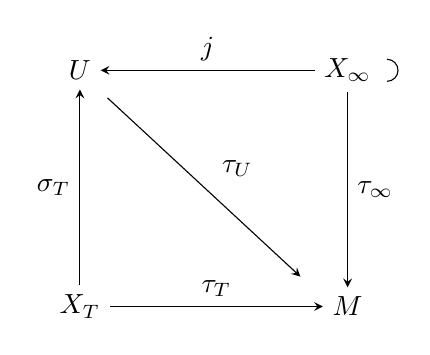
\begin{tikzpicture}[>=stealth]
  \node (U) at (0,0) {$U$};
  \node (Xi) at (3.4,0) {$X_{\infty}$};
  \node (XT) at (0,-3) {$X_{T}$};
  \node (M) at (3.4,-3) {$M$};
  \draw[->] (Xi) -- node[above]{$j$} (U);%
  \draw (3.9,0.14) arc (90:-90:0.14);%
  \draw[->] (0.35,-0.35) -- (2.8,-2.62);%
  \node at (2.0,-1.25) {$\tau_{U}$};
  \draw[->] (XT) -- node[left]{$\sigma_{T}$} (U);
  \draw[->] (Xi) -- node[right]{$\tau_{\infty}$} (M);
  \draw[->] (XT) -- node[above]{$\tau_{T}$} (M);
\end{tikzpicture}
\end{center}

其中映射 $\tau_{T}$、$\tau_{\infty}$ 与 $\tau_{U}$ 是在点 $(s,t)=(0,0)$ 处的%
赋值映射。现在设 $\tau_{T}^{*}$ 在上同调中是单射。那么 $\tau_{U}^{*}$ 也是单射，%
于是我们考虑\trAlexander-\trSpanier{}上同调的下述图表：

\begin{center}
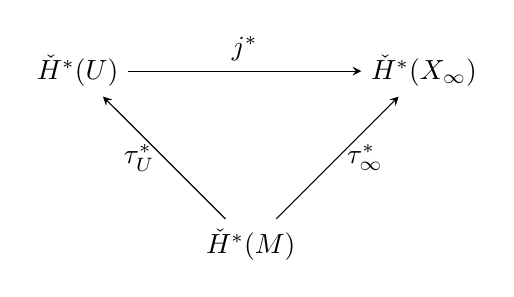
\begin{tikzpicture}[>=stealth]
  \node (HU) at (0,0) {$\check{H}^{*}(U)$};
  \node (HX) at (4.4,0) {$\check{H}^{*}(X_{\infty})$};
  \node (HM) at (2.2,-2.2) {$\check{H}^{*}(M)$};
  \draw[->] (HU) -- node[above]{$j^{*}$} (HX);
  \draw[->] (HM) -- node[right]{$\tau_{\infty}^{*}$} (HX);
  \draw[->] (HM) -- node[left]{$\tau_{U}^{*}$} (HU);
\end{tikzpicture}
\end{center}

鉴于\trAlexander-\trSpanier{}上同调的\trContinuity，我们可以对 $X_{\infty}$%
在 $C^{\infty}(\R\times S^{1},M)$ 中的一切开\trNeighborhood{} $U$ 取直极限，%
并得出映射 $\tau_{\infty}^{*}$ 是单射的。我们看到，有界解之集含有底\trManifold{}%
$M$ 的上同调；特别地，%
$\text{\trCupLength}\,(X_{\infty})\ \geq\ \text{\trCupLength}\,(M)$。把%
\trLjusternik-\trSchnirelman{}定理（\cref{thm:gradient-rest-points}）应用到%
$X_{\infty}$ 上的连续\trGradientLike\trFlow，我们便得出所要的陈述

\begin{theorem}[A.~\trFloer、H.~\trHofer]\label{thm:floer-hofer}
设 $(M,\omega)$ 是满足 $[\omega]\big|_{\pi_{2}(M)}=0$ 的\trCompact%
\trSymplecticManifold。那么 $M$ 上每个\trSmooth{}的时间\trPeriodic%
\trHamiltonianVectorField{} $\dot{x}=X_{H}(x)$ 都拥有至少%
$\text{\trCupLength}\,(M)+1$ 个周期为 $1$ 的可缩\trPeriodicSolution。
\end{theorem}

为完成\cref{thm:floer-hofer}的证明，我们尚须验证映射 $\tau_{T}^{*}$ 是单射。%
照 6.2 节的样子，我们将使用\trFredholm{}理论，以维数为 $2n$ 的\trSmooth%
\trCompact\trManifold{}逼近 $X_{T}$，其上同调可以用度理论来估计。下文中我们取定%
一个数 $T>5$，并把\trOperator{} $L=L^{T}$ 视为\trBundle
\[
L^{p}\Bigl(W^{1,p}(S_{T},M)^{*}A_{M}\Bigr)\ =\ \bigcup_{v\in W^{1,p}(S_{T},M)}\bigl\{v\bigr\}\times L^{p}\bigl(v^{*}A_{M}\bigr)\,.
\]
（底为 $W^{1,p}(S_{T},M)$）的一个\trSmooth\trSection。我们把这个\trBundle{}缩记为
\[
\mathcal{E}\ \to\ \mathcal{B}\,.
\]
现在的想法是：借同伦 $\rho\mapsto L_{\rho}$（$0\leq\rho\leq1$）把给定的%
\trSection{} $L$ 同伦于\trCauchy-\trRiemann{}型的\trSection{}%
$\frac{\partial}{\partial s}+J\frac{\partial}{\partial t}$，其中
\[
L_{\rho}(v)\ =\ Tv\ +\ J(v)(Tv)j\ +\ \rho\,\chi(s)\bigl[H'(t,v)\,ds\,-\,J(v)H'(t,v)\,dt\bigr]\,.
\]
引入赋值映射 $\tau:\mathcal{B}\to M$，$v\mapsto v(0,0)$，我们定义相伴的同伦%
$\hat{L}_{\rho}$（$0\leq\rho\leq1$）为
\[
\hat{L}_{\rho}(v)\ =\ \Bigl(L_{\rho}(v)\,,\,\tau(v)\Bigr)\,,\qquad 0\leq\rho\leq1\,.
\]
按定义，对每个 $0\leq\rho\leq1$ 这都是从 $\mathcal{B}$ 到 $\mathcal{E}\times M$%
的映射。我们可以把 $\mathcal{E}\times M$ 视为 $\mathcal{B}$ 之上的一个%
\trBanach{}流形丛。对 $\rho=0$，方程 $\hat{L}_{0}(v)=(0,m)$（给定 $m\in M$）%
只有常值解 $v_{0}\equiv m$，因为假设 $[\omega]\big|_{\pi_{2}(M)}=0$%
排除了非平凡的\trHolomorphic{}球面。在这个常值解%
（映射）$v_{0}$ 处的\trLinearization{}在第一个分量给出线性%
\trCauchy-\trRiemann\trOperator，在第二个分量给出在 $0$ 处的赋值。说得更精确些，%
以 $D=\hat{L}'_{0}(v_{0})$ 表示在特定点 $v_{0}\equiv m$ 处的\trLinearization，%
可以算得
\[
Dh\ =\ \Bigl(Th\ +\ J(m)(Th)j\,,\ h(0)\Bigr)\,.
\]
鉴于附录 4 中的结果，\trOperator{}%
$D:W^{1,p}(S_{T},T_{m}M)\to L^{p}(v_{0}^{*}A_{M})\times T_{m}M$ 是一个同构。现在%
我们对\trFredholm{}指数为零的\trFredholm{}截面使用 $\Z_{2}$-度。在必要的%
\trCompactness{}条件下，我们刚刚证明了这一度等于 $1$。让我们暂且假设%
$L_{\rho}(v)=0$（$0\leq\rho\leq1$）的解之集是\trCompact{}的。那么存在这个解集的%
一个开\trNeighborhood，\trFredholm{}映射限制在此\trNeighborhood{}上是恰当的，参见 S.~\trSmale{} [201]。%
于是，由 $\Z_{2}$-度的同伦性质，$\rho=1$ 时的原映射%
$v\mapsto\bigl(L_{1}(v),\tau(v)\bigr)$ 也具有等于 $1$ 的 $\Z_{2}$-度。为继续我们的%
思路，让我们再暂且假设映射 $v\mapsto L_{1}(v)$ 的像与\trBundle{} $\mathcal{E}$ 的%
\trZeroSection{} $0_{\mathcal{E}}$ \trTransversal。那么 $0_{\mathcal{E}}$ 的原像是%
$\mathcal{B}$ 的一张维数为 $2n$ 的\trSmooth\trCompact\trSubmanifold{} $\Sigma$。%
此外，由 $v\mapsto v(0,0)$ 定义的赋值映射%
$\tau:=\tau\big|_{\Sigma}:\Sigma\to M$ 将具有等于 $1$ 的 $\Z_{2}$-映射度。这使%
我们得以完全照 6.2 节中的\cref{prop:rho-injective-xt}的样子进行论证，证明%
$\tau_{T}^{*}$ 在\trAlexander-\trSpanier{}上同调中如愿是单射，从而完成%
\cref{thm:floer-hofer}的证明。为达到这一结论，我们假定了全部必要的%
\trCompactness，此外还假定了映射 $v\mapsto L_{1}(v)$ 的像与\trZeroSection%
$0_{\mathcal{E}}$ 的\trTransversality。这一\trTransversality{}可以通过对%
\trHamiltonianFunction{} $H$ 的一个任意 $C^{\infty}$-小\trPerturbation{}来建立。%
然而，这个论证相当精巧，关于证明我们请读者参见 A.~\trFloer、H.~\trHofer{}与%
D.~\trSalamon{} [87]。于是，有了这一\trPerturbation{}论证，再加上%
\trAlexander-\trSpanier{}上同调的\trContinuity，剩下的就只有%
\trCompactness{}问题了，尚须证明下述

\begin{proposition}\label{prop:xthat-compact}
设 $2<p<\infty$ 且 $[\omega]\big|_{\pi_{2}(M)}=0$。那么解之集
\[
\hat{X}_{T}:=\Bigl\{\,(\rho,v)\in[0,1]\times W^{1,p}(S_{T},M)\ \Bigm|\ L_{\rho}(v)=0\,\Bigr\}
\]
在 $[0,1]\times W^{1,p}(S_{T},M)$ 中是\trCompact{}的。
\end{proposition}

\begin{proof}[\cref*{prop:xthat-compact}的证明]
若 $v\in\hat{X}_{T}$，我们定义数 $\varepsilon(v)\geq0$ 为
\begin{equation}\label{eq:ell-epsilon-def}
\varepsilon(v)\ =\ \inf\Bigl\{\,\varepsilon>0\ \Bigm|\ \text{存在 }z\in S_{T}\ \text{满足 }\ \bigl|\nabla v\bigr|_{p,B_{\varepsilon}(z)}\ =\ \varepsilon^{\frac{2-p}{p}}\Bigr\}\,.
\end{equation}
此处 $B_{\varepsilon}(z)$ 表示 $S_{T}$ 上对某个固定度量而言围绕 $z$ 的%
$\varepsilon$-球。（由于 $S_{T}$ \trCompact，度量的选择无关紧要。）注意，函数%
$\varepsilon\mapsto\varepsilon^{\frac{p-2}{p}}\bigl|\nabla v\bigr|_{p,B_{\varepsilon}(z)}$%
不减。现在设
\[
\inf_{v\in\hat{X}_{T}}\ \varepsilon(v)\ \equiv\ \varepsilon>0\,.
\]
那么
\[
\bigl|\nabla v\bigr|_{p,B_{\varepsilon}(z)}\ \leq\ \varepsilon^{\frac{2-p}{p}}\text{\footnote{原书印作「$\bigl|\nabla v\bigr|_{p,B_{\varepsilon}(v)}(z)$」，把球心 $z$ 误置于范数记号之外、又以 $v$ 充当球心，依 \eqref{eq:ell-epsilon-def} 当为「$\bigl|\nabla v\bigr|_{p,B_{\varepsilon}(z)}$」，此处径改。——译者注}}
\]
对每个 $z\in S_{T}$ 成立，从而我们有 $\hat{X}_{T}$ 的一个 $W^{1,p}$-界。正如我们%
接下来要证明的，这个界蕴含 $\hat{X}_{T}$ 在 $[0,1]\times W^{1,p}(S_{T},M)$ 中的%
\trCompactness。把 $M$ 视为某个 $\R^{N}$ 的子集，我们可以把 $W^{1,p}(S_{T},M)$%
视为 $W^{1,p}(S_{T},\R^{N})$ 的子集。取序列 $(\rho_{k},v_{k})\in\hat{X}_{T}$；%
那么我们必须找出一个收敛子序列。取合适的子序列后，我们可以假设 $\rho_{k}\to\rho$，%
并且 $v_{k}\to v$（于 $C^{0}(S_{T},\R^{N})$ 中；鉴于\trCompact{}嵌入%
$W^{1,p}(S_{T},\R^{N})\subset C^{0}(S_{T},\R^{N})$），且 $v_{k}\rightharpoonup v$%
弱收敛于 $W^{1,p}(S_{T},\R^{N})$ 中（对某个 $v\in W^{1,p}(S_{T},\R^{N})$；鉴于%
空间 $W^{1,p}(S_{T},\R^{N})$ 的自反性）。我们将证明 $v_{k}$ 是%
$W^{1,p}(S_{T},\R^{N})$ 中的柯西序列。既然在 $C^{0}(S_{T},\R^{N})$ 中已有收敛，%
我们现在可以在 $S_{T}$ 与 $M$ 的\trChart{}中局部地进行。可能出现的任何困难都只%
发生在\trCylinder{} $Z_{T}\subset S_{T}$ 的\trBoundary{} $\partial Z_{T}\subset S_{T}$%
附近，因为在这个\trBoundary{}之外，诸映射 $u\in\hat{X}_{T}$ 是\trSmooth{}的（由%
椭圆正则性理论），因此我们可以像上面那样建立 $C^{\infty}$-界。于是我们只对最坏的%
情形实施局部论证，聚焦于 $S_{T}$ 的下\trCapDisk。为了在属于下\trCapDisk{}的\trBoundary{}%
$\partial Z_{T}$ 附近找到 $S_{T}$ 上的局部坐标，取一个双\trHolomorphic{}嵌入%
$\varphi:[-1,1]\times S^{1}\to S_{T}$，满足：对一切 $0\leq s\leq1$ 有%
$\varphi(s,t)=(s-T,t)$。现在在 $M$ 上选取\trSymplecticCoordinates，我们便面对%
如下局面。我们有映射序列 $v_{k}\in W^{1,p}\bigl(B_{\varepsilon}(0),\R^{2n}\bigr)$%
与数列 $\rho_{k}\in[0,1]$，满足
\[
\begin{aligned}
&v_{k}\ \longrightarrow\ v\qquad\text{于}\ C^{0}\Bigl(B_{\varepsilon}(0),\R^{2n}\Bigr)\ \text{中}\\
&v_{k}\ \ \rightharpoonup\ \ v\qquad\text{于}\ W^{1,p}\Bigl(B_{\varepsilon}(0),\R^{2n}\Bigr)\ \text{中}\\
&\rho_{k}\ \longrightarrow\ \rho\ \,,
\end{aligned}
\]
其中 $v\in W^{1,p}\bigl(B_{\varepsilon}(0),\R^{2n}\bigr)$，$v(0)=0$，而%
$B_{\varepsilon}(0)\subset\R^{2}$ 是以 $(s,t)=(0,0)$ 为中心的开\trDisc。此外，%
这些映射满足下述一阶椭圆\trPartialDifferentialEquation{}组
\[
\frac{\partial v_{k}}{\partial s}\ +\ J(v_{k})\frac{\partial v_{k}}{\partial t}\ +\ \rho_{k}\chi(s)H'(t,v_{k})\ =\ 0
\]
于 $B_{\varepsilon}(0)$ 上，此处 $\chi$ 是 $s$ 的正半直线的示性函数。我们得出：%
$v$ 满足方程
\[
\frac{\partial v}{\partial s}\ +\ J(v)\frac{\partial v}{\partial t}\ +\ \rho\,\chi(s)H'(t,v)\ =\ 0\,.
\]
我们将证明：对某个小的 $\delta>0$，$v_{k}$ 是%
$W^{1,p}\bigl(B_{\delta}(0),\R^{2n}\bigr)$ 中的柯西序列。设 $\beta:\R^{2}\to[0,1]$%
是一个\trSmooth{}函数，其\trSupport{}含于单位\trDisc，且在半径为 $\frac{1}{2}$%
的较小\trDisc{}上取值 $1$。对 $\tau>0$ 我们定义 $\R^{2}$ 上的函数 $\beta_{\tau}$%
为 $\beta_{\tau}(z)=\beta(z/\tau)$。以 $J_{0}$ 表示 $\R^{2n}$ 上的常值%
\trAlmostComplexStructure{} $J(0)$。最后，我们对 $\R^{2}$ 中的 $\varepsilon$-\trDisc%
上的 $W^{j,p}$-\trNorm{}写出 $|\cdot|_{j}$，回忆 $2<p<\infty$ 已固定。若%
$0<\tau<\varepsilon$，利用\trCauchy-\trRiemann\trOperator{}的经典估计%
\eqref{eq:ell-cr-estimate}，我们现在计算
\[
\begin{aligned}
c\,\bigl|\beta_{\tau}(v_{k}-v)\bigr|_{1}\ &\leq\ \bigl|\bar{\partial}\bigl(\beta_{\tau}(v_{k}-v)\bigr)\bigr|_{0}\\
&\leq\ \Bigl|\frac{\partial}{\partial s}\bigl(\beta_{\tau}(v_{k}-v)\bigr)\ +\ J(v)\frac{\partial}{\partial t}\bigl(\beta_{\tau}(v_{k}-v)\bigr)\Bigr|_{0}\\
&\qquad+\ \bigl|J_{0}-J(v)\bigr|_{L^{\infty}(B_{\tau})}\,\bigl|\beta_{\tau}(v_{k}-v)\bigr|_{1}\\
&\leq\ \Bigl|\beta_{\tau}\Bigl(\frac{\partial}{\partial s}(v_{k}-v)\ +\ J(v)\frac{\partial}{\partial t}(v_{k}-v)\Bigr)\Bigr|_{0}\ +\ c_{1}(\tau)\bigl|v_{k}-v\bigr|_{0}\\
&\qquad+\ \sigma(\tau)\bigl|\beta_{\tau}(v_{k}-v)\bigr|_{1}\,.
\end{aligned}
\]
此处当 $\tau\to0$ 时 $\sigma(\tau)\to0$，而 $c_{1}(\tau)$ 是依赖于 $\tau$ 的%
常数。于是，若 $\tau>0$ 充分小，
\begin{align*}
\frac{c}{2}\,\bigl|\beta_{\tau}(v_{k}-v)\bigr|_{1}\ &\leq\ c_{1}(\tau)\bigl|v_{k}-v\bigr|_{0}\ +\ \bigl|J(v)-J(v_{k})\bigr|_{L^{\infty}(B_{\tau})}\,\bigl|v_{k}\bigr|_{1}\\
&\quad+\ \Bigl|\rho_{k}\chi H'(t,v_{k})\ -\ \rho\chi H'(t,v)\Bigr|_{0}\,.
\end{align*}
由假设，$\bigl|v_{k}\bigr|_{1}$ 是有界序列，$\bigl|v_{k}-v\bigr|_{0}\to0$，%
$J(v_{k})\to J(v)$ 在 $B_{\varepsilon}(0)$ 上一致，且%
$\bigl|\rho_{k}\chi H'(t,v_{k})-\rho\chi H'(t,v)\bigr|_{0}\to0$\footnote{原书此式首项印作「$\rho_{k}H'(t,v_{k})$」，脱 $\chi$——本段偏微分方程与上一估计式中该项均作 $\rho_{k}\chi H'(t,v_{k})$，无 $\chi$ 则收敛式在 $\chi=0$ 区域不立——此处径补。——译者注}。于是%
$v_{k}\to v$（于 $W^{1,p}\bigl(B_{\delta}(0),\R^{2n}\bigr)$ 中），对某个充分小的%
$\delta>0$。用有限多个\trChart{}覆盖 $S_{T}$，我们便证明了 $v_{k}\to v$（于%
$W^{1,p}(S_{T},M)$ 中），从而 $\hat{X}_{T}$ \trCompact，正如命题所断言。

为结束我们的论证，尚须验证我们的假设：数 $\varepsilon(v)$ 在集合%
$\hat{X}_{T}$ 上一致地不趋近 $0$。我们反证：假设 $\hat{X}_{T}$ 没有一致的%
$W^{1,p}$-界，那么可以找到序列 $(\rho_{k},v_{k})\in\hat{X}_{T}$ 满足%
$\varepsilon(v_{k})\to0$。由 $\varepsilon(v)$ 的定义，我们可以找到序列%
$z_{k}\in S_{T}$，使得取 $\varepsilon_{k}:=\varepsilon(v_{k})$ 便有
\[
\bigl|\nabla v_{k}\bigr|_{0,B_{\varepsilon_{k}}(z)}\ \leq\ \bigl|\nabla v_{k}\bigr|_{0,B_{\varepsilon_{k}}(z_{k})}
\]
对一切 $z\in S_{T}$。此外，
\[
1\ =\ \varepsilon_{k}^{\frac{p-2}{p}}\ \bigl|\nabla v_{k}\bigr|_{0,B_{\varepsilon_{k}}(z_{k})}\,.
\]
由于 $\varepsilon_{k}\to0$，并且由于在远离 $\partial Z_{T}$ 处我们有%
$C^{\infty}$ 界，我们推出 $\operatorname{dist}(z_{k},\partial Z_{T})\to0$。于是，%
取子序列后可以假设 $z_{k}\to z_{0}\in\partial Z_{T}$。现在的论证类似于前面%
\trBubblingOffAnalysis{}中所用者。就是说，我们在 $z_{k}$ 附近重新标度，从而得到%
一个具有 $W^{1,p}_{\mathrm{loc}}$-界的新序列。于是，照上面那样论证，新序列%
$u_{k}$ 将是 $W^{1,p}_{\mathrm{loc}}$-\trPrecompact{}的。从而取一个合适的子序列后，%
我们可以取极限，得到方程 $v_{s}+J(v)v_{t}=0$ 在 $\C$ 上的一个非常值解%
$v\in W^{1,p}(\C,M)$\footnote{原书印作「a nonzero solution」（非零解），然流形%
$M$ 并无零元可指，依上下文当为「非常值解」（nonconstant solution）之误，%
此处径改。——译者注}。由椭圆正则性理论，$v\in C^{\infty}(\C,M)$。此外，%
$\int_{\R^{2}}\bigl|\nabla v\bigr|^{2}_{J}\,ds\,dt<\infty$\footnote{原书积分域%
印作「$\int_{\R}$」，然 $v$ 是刚得到的、定义在 $\C\cong\R^{2}$ 上的重标度极限，%
二维积分域当为「$\R^{2}$」（旧注所猜「$\R\times S^{1}$ 之省」与此局部起泡极限%
不符，一并订正），此处径改。——译者注}；这由%
\eqref{eq:ell-limit-energy} 应用到我们的序列 $u_{k}$，再加上下述\trCapDisk{}的先验估计%
而得出：
\[
\Bigl|\ \int_{D}u_{k}^{*}\omega\Bigr|\ \leq\ 2C\,,
\]
后者立刻由\cref{lem:action-tube-bound}之前的那个估计得出。现在照%
\cref{thm:gradient-estimate} 的证明那样论证，我们就与拓扑假设%
$[\omega]\big|_{\pi_{2}(M)}=0$ 相矛盾。\cref{prop:xthat-compact}的证明、从而%
\cref{thm:floer-hofer} 的证明到此完成。
\end{proof}


\textbf{\trhRemark。}\quad 我们注意到，\trTorus{} $(T^{2n},\omega)$ 对每个%
\trSymplecticStructure{} $\omega$ 都满足\cref{thm:floer-hofer}的假设。

\cref{thm:floer-hofer}归功于 A.~\trFloer{} [86] 与 H.~\trHofer{} [115]（1987 年）。%
两人都是从一个关于\trCompact{}拉格朗日\trManifold{}的更一般的\trIntersection{}结果导出该%
结果。M.~\trChaperon{}在其\trBourbaki{}讲演 [42]（1982--83）中便已注意到，%
\trVariational{}进路可适用于 V.~I.~\trArnold{}在 [9] 中所提示的拉格朗日%
\trManifold{}的整体\trIntersection{}问题。

上述断言中的\trCohomology{}取 $\Z_{2}$ 系数；我们想指出，该断言实际上对每个%
\trCoefficientField{}都成立。然而，其证明需要来自\trFredholm{}理论与\trAlgebraicTopology{}的更为精细的%
工具。关键之处在于为一类特定的\trFredholm{}算子解决若干\trOrientation{}问题。%
关于所涉及的技术，我们请读者参见 A.~\trFloer{}与 H.~\trHofer{} [89]。结果表明，%
只要 $X_{T}$ 是\trManifold，它便带有从 $(M,\omega)$ 的\trOrientation{}继承而来%
的一个自然定向。

对一般\trSymplecticManifold{} $(M,\omega)$ 的\trArnold{}猜想的上述证明，%
至关重要地使用了要求 $[\omega]\big|_{\pi_{2}(M)}=0$ 的这一苛刻假设；我们指出，%
没有这一假设，该猜想仍未解决。然而，若（先验地）要求所考虑的%
\trHamiltonianVectorField{}的全部 $1$-\trPeriodicSolution{}都\trNondegenerate，%
则还能多说一些，正如我们将在下一节看到的。
